% =============================================================================
%  Imperial College London — MEng (AI & Machine Learning) Final Year Project
%  Structured Refactoring Agent for IntelliJ
%
%  Build:  cd report && latexmk -pdf main.tex     (or pdflatex x2 + bibtex)
%  This is a SCAFFOLD. Prose marked [WRITE: ...] is yours to author.
%  See WRITING_GUIDE.md for the page budget, rubric mapping, and day-by-day.
% =============================================================================
\documentclass[11pt,a4paper]{report}

\usepackage[utf8]{inputenc}
\usepackage[T1]{fontenc}
\usepackage{lmodern}   % scalable fonts (required by microtype expansion)
\usepackage[a4paper,margin=2.5cm]{geometry}
\usepackage{graphicx}
\usepackage{tikz}
\usetikzlibrary{positioning,arrows.meta}
\usepackage{booktabs}
\usepackage{amsmath}
\usepackage{xcolor}
\usepackage{listings}
\usepackage{microtype}
\usepackage[numbers,square]{natbib}
\usepackage{hyperref}
\usepackage{cleveref}   % load AFTER hyperref

\graphicspath{{figures/}}

% ---- Visible placeholder for content you still need to write -----------------
\newcommand{\writeme}[1]{\textcolor{red}{\textbf{[WRITE:} #1\textbf{]}}}

% ---- Code listing style ------------------------------------------------------
\definecolor{codegray}{gray}{0.95}
\lstdefinestyle{code}{
  backgroundcolor=\color{codegray},
  basicstyle=\ttfamily\footnotesize,
  breaklines=true,
  captionpos=b,
  frame=single,
  numbers=left,
  numberstyle=\tiny,
  showstringspaces=false,
  tabsize=2,
}
\lstset{style=code}

% ---- Project metadata (FILL THESE IN) ---------------------------------------
\newcommand{\reporttitle}{Structured Refactoring Agent for IntelliJ:\\Decoupling LLM Reasoning from AST-Safe Execution}
\newcommand{\reportauthor}{Ibrahim Ibrahim}
\newcommand{\supervisorname}{Dr Robert Chatley}
\newcommand{\secondmarkername}{\writeme{second marker name}}
\newcommand{\reportdate}{June 2026}

% NOTE: PDF metadata must be plain text — no \\ and no \writeme/\textcolor here.
\hypersetup{
  colorlinks=true, linkcolor=black, citecolor=black, urlcolor=blue,
  pdftitle={Structured Refactoring Agent for IntelliJ},
  pdfauthor={Ibrahim}
}

\begin{document}

% ============================== TITLE PAGE ===================================
\begin{titlepage}
  \centering
  \vspace*{1cm}
  {\scshape\LARGE Imperial College London \par}
  \vspace{0.3cm}
  {\scshape\large Department of Computing \par}
  \vspace{2.5cm}
  {\huge\bfseries \reporttitle \par}
  \vspace{2.5cm}
  {\Large \reportauthor \par}
  \vspace{0.2cm}
  {\large CID: 01870877 \par}
  \vspace{1cm}
  {\large Supervisor: \supervisorname \par}
  {\large Second Marker: \secondmarkername \par}
  \vfill
  {\large Submitted in partial fulfilment of the requirements for the\\
   MEng degree in Computing (Artificial Intelligence and Machine Learning)\par}
  \vspace{1cm}
  {\large \reportdate \par}
\end{titlepage}

% ============================== ABSTRACT =====================================
\chapter*{Abstract}
\addcontentsline{toc}{chapter}{Abstract}
% ~250 words. Write this LAST, once results are final.
% Must state: problem, what you built, what you measured, the headline result.
Large language models can reliably identify useful refactorings but apply them
unreliably: when an LLM rewrites source text directly it misses cross-file usages,
breaks imports, and produces changes that compile yet are semantically wrong, with the
strongest models reaching only about 41.6\% on repository-level refactoring benchmarks.
This project argues that the limitation lies in the \emph{action space} rather than the
model, and addresses it by decoupling reasoning from execution. An IntelliJ~IDEA plugin
exposes the IDE's PSI-backed refactoring engine --- rename, move, change-signature,
safe-delete, inline, extract, and symbol creation --- as a model-agnostic,
externally-callable tool API, over HTTP and the Model Context Protocol, that any
function-calling agent can drive. Because every edit is performed by the IDE engine
rather than emitted as text, each change is behaviour-preserving and propagated across
the whole codebase by construction.

The system is evaluated with a controlled comparison that holds the model fixed and
varies only the edit primitive, across three real-world Java projects (spring-petclinic,
Apache Commons Lang, and jackson-databind, up to 474 source files), scored by
compilation and disk-state checks. The result is deliberately nuanced: against scripted
and weak-model text baselines the structured engine wins clearly (9/9 versus 6/9 on
spring-petclinic), but a \emph{capable} agent editing raw text reaches parity on
behaviour-preserving refactorings (12 of 12 across the three projects). The structured
action space's durable, measured advantages are therefore correctness \emph{by
construction} --- independent of the model's capability and of any build-feedback loop
--- exhaustive, type-aware structural queries that text editing cannot perform at all,
and far fewer mutating operations; advantages that prove decisive precisely where the
driving agent is weak, scripted, or unverified.

% ============================== DECLARATION ==================================
\chapter*{Declarations}
\addcontentsline{toc}{chapter}{Declarations}

\noindent\textbf{Originality.}\\
% This must be YOUR honest statement. Template only.
This report and the work it describes are my own, except where explicitly stated and
referenced.

\vspace{1em}
\noindent\textbf{Source code.}\\
The implementation is available at:
\url{https://github.com/ibrahim-io/structured-refactoring-agent-intellij}.
% NOTE (rubric requirement): the repo link goes here AND your supervisor must
% have been granted access to the repository.

\vspace{1em}
\noindent\textbf{Use of generative AI.}\\
% CRITICAL — see WRITING_GUIDE.md. Undeclared/over-relied-upon AI => 0-39% cap
% + possible misconduct referral. Acceptable use (coding assistance, structuring,
% proofreading) is fine IF disclosed, human-reviewed, and you remain the author.
% Write this honestly and specifically. Template prompts below — REPLACE them.
This project made substantial and disclosed use of generative AI --- specifically
Anthropic's Claude (the Claude Opus~4.8 model, used through the Claude Code agentic
command-line tool) --- in three roles. First, as a \emph{coding assistant} for parts of
the plugin and the evaluation harness, including the headless-execution technique and
the benchmark runners. Second, in \emph{writing}: to produce first drafts and structure
for this report from my own research notes, design decisions, and measured results,
which I then reviewed, corrected, rewrote where necessary, and verified against the
source code and the data. Third, in the \emph{evaluation itself}: Claude was used both
to orchestrate the benchmark runs and, in the controlled comparison
(\Cref{sec:eval-controlled}), as the ``capable agent'' under test that drives the
refactoring tools; this dual role is stated explicitly in the methodology, and means
that arm demonstrates the system's intended deployment rather than an independent
third-party benchmark. I directed the work throughout, I checked the factual claims,
figures, and citations myself, and I am the author of both the system and this report;
all AI-generated text and code was reviewed and adapted by me rather than submitted as
produced, and I can explain and defend every part.

\vspace{1em}
\noindent\textbf{Ethics.}\\
This project involved neither human participants nor personal data: it is a software
system evaluated entirely on open-source code repositories. The developer study
originally considered as an extension was not conducted, so the project required no
ethics approval.

% ============================ ACKNOWLEDGEMENTS ================================
\chapter*{Acknowledgements}
\addcontentsline{toc}{chapter}{Acknowledgements}
I am grateful to my supervisor, Dr Robert Chatley, for his guidance and feedback
throughout this project, and for the freedom to pursue the direction it took. I
would also like to thank my family and friends for their support over the course
of my degree at Imperial College London.

% ============================== CONTENTS =====================================
\tableofcontents
\listoffigures
\listoftables

% ============================== CHAPTERS =====================================
% =============================================================================
%  CHAPTER 1 — INTRODUCTION
%
%  >>> MOTIVATION + REPORT STRUCTURE are an AI-ASSISTED FIRST DRAFT (from your
%      docs/PROJECT_CONTEXT.md + RELATED_WORK.md). Rewrite in your own voice,
%      verify citations, and disclose in the Declarations page.
%  >>> OBJECTIVES, RESEARCH-QUESTION FRAMING, and CONTRIBUTIONS are left for YOU
%      — they are your claims and the heart of the Framing mark (15%). I'll edit
%      what you write, but these should not be ghost-drafted.
%  RUBRIC: Framing of Research Problem (15%). BUDGET: ~4-6 pages.
% =============================================================================
\chapter{Introduction}
\label{ch:intro}

\section{Motivation}
\label{sec:intro-motivation}

Software spends most of its life being maintained rather than written, and a
large share of that maintenance is \emph{refactoring}: behaviour-preserving
restructuring that keeps a codebase readable and able to evolve. The arrival of
capable large language models (LLMs) inside the IDE has changed how developers
approach such work --- controlled studies report that AI pair-programmers let
developers complete tasks substantially faster \citep{copilotproductivity2023}
--- and LLMs are now demonstrably able to \emph{identify} useful refactorings
and describe how to carry them out \citep{cordeiro2024refactoring,
potentialllm2024}.

The difficulty lies not in deciding \emph{what} to refactor but in
\emph{applying} the change correctly. When an LLM performs a refactoring by
generating modified source text, it must itself locate and update every affected
site. In practice it routinely misses usages in other files
(\emph{scope blindness}), breaks import statements, introduces compilation
errors, or produces code that compiles but is semantically wrong
\citep{llmrefactorlimits2025}. These are not occasional lapses: on a
repository-level benchmark of 1{,}099 real, behaviour-preserving Java
refactorings, the strongest evaluated LLM reaches a pass rate of only 41.6\%
\citep{swerefactor2025}. The model is reliable at \emph{what} and unreliable at
\emph{how} --- precisely because ``how'' has been framed as the problem of
writing correct code text.

Yet that problem is already solved, just not by the model. Every modern IDE
contains a refactoring engine that performs renames, moves, signature changes,
and extractions over a typed program model, updating all references, imports,
and occurrences atomically and correctly by construction. The weakness of
current LLM agents is that they do not use it for writes: agent toolkits expose a
general-purpose textual \texttt{edit} action \citep{sweagent2024}, and even
systems that exploit the abstract syntax tree do so only to \emph{read} context
before emitting a text patch \citep{autocoderover2024}. Where the IDE engine
\emph{is} used for execution, as in EM-Assist \citep{emassist2024}, it is wired
to a single operation inside the IDE, with no interface an external agent could
call.

This project argues that an LLM agent should be \emph{decoupled} from the act of
writing code: the model should decide \emph{what} to refactor, and the IDE's
refactoring engine should decide and execute \emph{how}. Concretely, it presents
an IntelliJ~IDEA plugin that exposes the IDE's structured refactoring operations
--- rename, move, change-signature, safe-delete, inline, extract, and symbol
creation --- through a localhost tool API that any function-calling LLM can
drive. Because every mutation is performed by IntelliJ's PSI engine rather than
by text substitution, the result is correct with respect to the IDE's semantic
model independently of the quality of the model's textual output.
This report defends a single claim: that the IDE's structured operations are a
better action space for an LLM refactoring agent than source text --- not because
a capable model cannot edit text correctly, but because routing every edit
through IntelliJ's PSI engine makes project-wide, behaviour-preserving refactoring
of real-world Java codebases correct \emph{by construction} and more efficient,
and uniquely supports the project-wide structural queries (such as exhaustive
reference finding) that text editing cannot perform. The advantage is largest
exactly where text editing is least reliable: under weaker models, and for
refactorings whose correctness depends on a project-wide reference or type graph.

\section{Objectives}
\label{sec:intro-objectives}
% YOUR SECTION. Turn your research questions (docs/EVALUATION.md) into explicit,
% testable objectives. List only what the evaluation actually measures; move the
% developer study (RQ4) to Future Work if you do not run it.
This project pursues four objectives, each phrased so that it is tested directly
by the evaluation in Chapter~\ref{ch:eval}.

\begin{enumerate}
  \item \textbf{Expose the IDE's refactoring engine as an agent action space.}
  Design and implement an IntelliJ~IDEA plugin that makes the platform's
  PSI-backed operations --- rename, move, change-signature, safe-delete, inline,
  extract, and symbol creation --- callable by an external function-calling LLM
  through a localhost tool API.
  \emph{(Substantiated in Chapters~\ref{ch:design}--\ref{ch:impl}.)}

  \item \textbf{Demonstrate behaviour-preserving correctness on real-world code.}
  Show that refactorings executed through this action space are applied
  correctly on two real-world Java projects (spring-petclinic and Apache Commons
  Lang), measured by per-task pass rate under compilation and symbol-survival
  checks. \emph{(Chapter~\ref{ch:eval}.)}

  \item \textbf{Establish where structured execution is \emph{necessary}.}
  Isolate and measure the refactoring classes on which text-level editing fails
  --- cross-file moves requiring import repair, overload-safe and cross-class
  renames, and project-wide usage discovery --- to show where the structured
  approach is not merely tidier but required for correctness.
  \emph{(Chapter~\ref{ch:eval}, root-cause analysis.)}

  \item \textbf{Compare against a text-editing baseline.}
  Evaluate the structured approach against both a scripted text editor and an LLM
  text-edit agent on the same tasks, comparing correctness and the minimality of
  the resulting diffs. \emph{(Chapter~\ref{ch:eval}.)}
\end{enumerate}

\section{Research-Question Framing}
\label{sec:intro-rqs}
% YOUR SECTION. Frame the work as AI-systems research, not just a plugin: e.g.
% "how should an LLM agent's action space be designed for safe, reliable,
% project-wide code transformation?" Cite the ACI abstraction \citep{sweagent2024}
% and the constrained-action-space taxonomy \citep{demystifying2025}.
We frame this work not as a plugin but as a question about \emph{agent design}.
Under the agent--computer-interface (ACI) abstraction \citep{sweagent2024}, an
LLM agent's competence is governed less by raw model capability than by the
\emph{action space} it is given --- the set of operations through which it
observes and changes the world; recent analysis of code agents makes the same
point, treating the design of a constrained, well-typed action space as a
primary determinant of reliability \citep{demystifying2025}. Conventional coding
agents take \emph{source text} as their action space. This work asks what
changes when the action space is instead the IDE's structured refactoring
engine:

\begin{description}
  \item[RQ1 (Correctness).] Does constraining an agent's action space to the
  IDE's structured, AST-aware refactoring operations --- rather than free-form
  text edits --- improve the correctness of behaviour-preserving, project-wide
  refactorings on real-world codebases? \emph{(Objectives~2, 4.)}

  \item[RQ2 (Necessity).] For which classes of refactoring is a structured
  action space not merely beneficial but \emph{necessary} --- i.e.\ where does
  text-level editing fail for reasons intrinsic to its action representation
  rather than to model capability? \emph{(Objective~3.)}

  \item[RQ3 (Cost).] What does this safety cost? Does routing every edit through
  the IDE engine change the minimality of the resulting diffs and the agent's
  interaction cost (tool calls and turns) relative to a text-editing agent?
  \emph{(Objective~4.)}
\end{description}

\section{Contributions}
\label{sec:intro-contributions}
% YOUR SECTION. Adapt the novelty claims in docs/PROJECT_CONTEXT.md, but HEDGE
% absolute "first/only" claims to "to the best of our knowledge" and acknowledge
% contemporaneous work (e.g. the JetBrains MCP server). Each contribution should
% map to a chapter/section.
The contributions of this report are:

\begin{enumerate}
  \item \textbf{A structured-refactoring tool API for LLM agents.} An
  IntelliJ~IDEA plugin that exposes the platform's PSI-backed refactoring
  operations through a model-agnostic, function-calling HTTP interface, letting
  an external LLM \emph{execute} --- not merely propose --- project-wide
  refactorings. To the best of our knowledge this is the first general-purpose
  interface of its kind for arbitrary function-calling agents; it is
  contemporaneous with, and complementary to, the JetBrains MCP server.
  \emph{(Chapters~\ref{ch:design}--\ref{ch:impl}.)}

  \item \textbf{A headless-execution technique for IDE refactorings.} A method
  for making \texttt{BaseRefactoringProcessor}-based refactorings fully
  non-interactive --- suppressing the preview, conflict, and error dialogs that
  otherwise block an unattended IDE --- so that an agent can drive them without
  a human at the keyboard. \emph{(Chapter~\ref{ch:impl}.)}

  \item \textbf{An evaluation methodology and benchmark.} A reproducible harness
  that compares structured execution against both a scripted text editor and an
  LLM text-edit agent on real-world Java projects, scoring correctness
  (compilation and symbol survival) and diff minimality.
  \emph{(Chapter~\ref{ch:eval}.)}

  \item \textbf{An empirical characterisation of where the action space matters.}
  Evidence that text-level editing fails on reference-graph- and type-dependent
  refactorings --- cross-file moves with import repair, overload-safe and cross-class
  renames, and project-wide usage discovery --- for scripted and weaker-model drivers;
  that a \emph{capable} agent reaches parity on those refactorings; and that the
  structured engine's durable advantages are therefore correctness by construction, the
  structural queries text editing cannot express, and robustness to the driver's
  capability. \emph{(Chapter~\ref{ch:eval}.)}
\end{enumerate}

\section{Report Structure}
\label{sec:intro-structure}

The remainder of this report is organised as follows.
Chapter~\ref{ch:background} reviews the relevant literature on LLM-driven
refactoring, program-transformation agents, AST-safe refactoring, and tool use,
and identifies the gap this work addresses.
Chapter~\ref{ch:design} presents the design: the decoupling of model reasoning
from IDE execution, the tool API, and the rationale behind the key design
decisions.
Chapter~\ref{ch:impl} describes the implementation, including how each operation
delegates to IntelliJ's refactoring engine and the principal engineering
challenges overcome.
Chapter~\ref{ch:eval} evaluates the system against a text-editing baseline on
two benchmark projects, reporting correctness, efficiency, and a root-cause
analysis of the baseline's failures.
Chapter~\ref{ch:conclusion} concludes with a reflection on the results, their
broader impact, and directions for future work.

% =============================================================================
%  CHAPTER 2 — BACKGROUND & RELATED WORK
%
%  >>> AI-ASSISTED FIRST DRAFT (generated from YOUR docs/RELATED_WORK.md). <<<
%  This is raw material, NOT submittable text. Before submission you MUST:
%    1. Rewrite it in your own voice (the markers quiz you on this in the viva).
%    2. Verify every citation against the actual paper — several entries in
%       references.bib are marked `VERIFY` (authors, venues, the SWE-Refactor ID
%       and its 41.6% figure, on which your motivation depends).
%    3. Disclose AI drafting assistance in the Declarations page (main.tex).
%  RUBRIC: Framing of Research Problem (15%). BUDGET: ~8-12 pages.
% =============================================================================
\chapter{Background and Related Work}
\label{ch:background}

\section{Technical Background}
\label{sec:bg-technical}

This section introduces the concepts a reader needs to follow the rest of the
report: the structural representation an IDE maintains for source code, the
refactoring engine that operates on it, and the tool-use mechanism by which a
large language model (LLM) can invoke external operations.

\paragraph{Program structure and the PSI.} Modern IDEs do not treat source code
as text. IntelliJ IDEA maintains a \emph{Program Structure Interface} (PSI): a
typed abstract syntax tree augmented with a project-wide reference index that
resolves each identifier to its declaration and each declaration to all of its
usages. Because the PSI encodes types, scopes, and references rather than
character offsets, an operation expressed over it can reason about \emph{which}
\texttt{addVisit} a call refers to, or \emph{which} overload of \texttt{getPet}
a signature selects --- information that is absent from the raw text.

\paragraph{Refactoring engines.} A refactoring is a behaviour-preserving
transformation of a program. IntelliJ implements each refactoring as a
\emph{processor} (e.g.\ \texttt{RenameProcessor},
\texttt{MoveClassesOrPackagesProcessor}, \texttt{ChangeSignatureProcessor})
that mutates the PSI and propagates the change to every dependent reference,
import, and --- where requested --- comment and string occurrence, atomically.
The correctness of the result follows from the engine's semantic model, not from
the caller. This is the foundation of the design: by constraining the agent to \emph{only}
drive these PSI-backed operations --- never to edit source text directly ---
correctness no longer depends on the agent's own reasoning about where a change
must ripple. The agent need only choose \emph{which} refactoring to apply; the
engine then guarantees that the rename, signature change, or move is
behaviour-preserving by definition, propagating to every dependent reference
across the codebase atomically and without the missed call sites, broken imports,
or other unintended side effects that ad hoc text editing risks.

\paragraph{LLM tool use and the Model Context Protocol.} Contemporary LLMs
support \emph{function calling}: given a set of named tools described by a JSON
schema, the model emits a structured call (a tool name and a JSON argument
object) that the host application executes, returning the result for the model
to continue reasoning. The Model Context Protocol (MCP) standardises this
exchange so that any compliant agent can discover and call a server's tools.
This project exposes IntelliJ's refactoring engine through exactly such a
tool interface.

\section{LLM-Driven Code Refactoring}
\label{sec:bg-llm-refactoring}

A growing body of work evaluates how well LLMs can be applied to software
engineering and code tasks; \citet{hou2024llm4se} provide a systematic literature
review of 395 such studies and identify interpretability and trustworthiness,
together with limited evaluation on industrial data, as open challenges that still
impede real-world adoption --- challenges that a structurally-safe,
behaviour-preserving execution layer is well placed to lower.
\citet{cordeiro2024refactoring} study StarCoder2 across thirty open-source Java
projects, and find that the model outperforms developers on systematic, repetitive
refactorings but falls short on context-heavy, architectural ones --- precisely the
cases that depend on project-wide reference information. \citet{potentialllm2024} examine 180
real-world refactorings across twenty projects and report that ChatGPT
identifies only 28 of them unaided, yet reaches an 86.7\% success rate once the
refactoring sub-category is pre-specified. This last result is important for the
present work: constraining the model to a fixed menu of operation types --- as a
typed tool API does --- substantially improves reliability over free-form
generation.

The clearest statement of the problem comes from repository-level benchmarks.
\citet{swerefactor2025} assemble 1{,}099 developer-written, behaviour-preserving
Java refactorings validated by compilation, tests, and RefactoringMiner, and
report a best LLM pass rate of only \textbf{41.6\%}. This ceiling on
text-generation approaches is the empirical motivation for delegating execution
to an IDE. Complementarily, \citet{llmrefactorlimits2025} catalogue the failure
modes behind that ceiling --- hallucinated edits, broken semantics, and
\emph{scope blindness} (missing usages in other files) --- and identify IDE
integration as the natural mitigation. This work targets the \emph{execution} step those failure modes share: it removes
free-text generation from the write path entirely, so the scope-blind,
semantically-unsafe edits behind that ceiling --- missed cross-file usages, broken
imports, wrong-overload renames --- cannot arise, because every change is applied by
an AST-aware engine that propagates it across the whole codebase by construction.

\section{Program Transformation Agents}
\label{sec:bg-agents}

A parallel line of work embeds LLMs in autonomous agents that act on a codebase
through a tool interface. \citet{sweagent2024} introduce the Agent--Computer
Interface (ACI): a small, shell-like toolset (view, search, edit, run) through
which an agent resolves real GitHub issues, achieving 12.5\% on SWE-bench at
release. The ACI is the closest architectural analogue to this project's HTTP
tool surface, but its \texttt{edit} tool performs raw text replacement with no
awareness of program structure. \citet{openhands2025} generalise this to a
sandboxed platform in which agents drive a containerised operating system
(shell, browser, Python REPL); the action space is maximally general but
correspondingly unconstrained. \citet{autocoderover2024} narrow the focus to
program repair, using AST-backed code-search APIs (class signatures, method
bodies, call graphs) to locate context before generating a patch; notably,
however, the AST is used only for \emph{read-only retrieval}, while the patch is
still applied as a text diff. Across this line of work the pattern is
consistent: structure, where used at all, informs \emph{reading}, never
\emph{writing}.

% --- AI FIRST DRAFT (from arXiv:2511.04824 + your research notes). Verify the
%     figures against the paper and edit into your voice. ---
The most direct empirical evidence for how such agents refactor in practice comes
from \citet{agenticrefactoring2025}, who conduct the first large-scale study of
production coding agents (Codex, Cursor, Devin, Claude Code), detecting 15{,}451
refactorings across 14{,}988 real Java commits with RefactoringMiner and assessing
their structural impact with DesigniteJava. Two of their findings directly motivate
the present work. First, although agents refactor in 26.1\% of commits, they
overwhelmingly perform \emph{localized, low-level} edits --- change-variable-type
(11.8\%), rename-parameter (10.4\%), and rename-variable (8.5\%) dominate --- a
``preference for localized improvements over the high-level design changes common
in human refactoring''. The structural operations agents largely avoid (move,
extract, signature change) are precisely those where free-text editing is least
safe, as the present evaluation confirms (\Cref{ch:eval}); a structured execution
layer is what makes them safe to attempt. Second, their quality analysis finds only
\emph{small} structural gains (e.g.\ a median reduction of 15.25 class lines of
code) and reports that agents ``fail to meaningfully reduce actual design
smells''; moreover 53.9\% of the detected refactorings occur in \emph{tangled}
commits with no explicit refactoring intent --- applied incidentally alongside
other edits rather than as deliberate, isolated transformations. The study does
not establish that these edits compile or preserve behaviour. These are precisely
the guarantees an IDE-backed execution layer provides by construction, and the
intentful, single-purpose nature of a typed refactoring operation is what makes
each change individually reviewable rather than entangled with unrelated edits.
This project therefore complements their descriptive account of \emph{what} agents
refactor with a prescriptive question: does constraining the agent's write action
to structured, semantics-preserving operations improve correctness, reproducibility,
and auditability?

\section{AST-Safe and Structured Refactoring with AI}
\label{sec:bg-structured}

The systems most closely related to this project combine an LLM with an IDE's
refactoring engine so that execution is structurally safe. \citet{emassist2024}
present EM-Assist, an IntelliJ plugin in which an LLM suggests code ranges to
extract and IntelliJ's PSI engine validates and performs the extraction,
reaching 53.4\% Recall@5 on 1{,}752 real refactorings with a 94.4\% positive
developer rating. EM-Assist is the most architecturally similar prior system and
the natural baseline for comparison; its limitation is that it is
\emph{single-operation} (extract-method only) and hardwired inside the IDE, with
no external interface an agent could call.
\citet{movemethod2025} combine LLM suggestions with IDE static analysis and
retrieval over prior refactorings to recommend Move Method, reaching 73\%
Recall@1 --- again a single operation, exposed through no agent-callable API.
\citet{mantra2025} orchestrate multiple LLM agents with contextual RAG and
self-repair across six method-level refactoring types (including extract-method),
with 82.8\% of generated refactorings compiling and passing tests overall; the
pipeline is sophisticated but still produces text-level replacements rather than
driving the IDE's engine.
A distinct, human-centred strand examines how developers and an LLM actually
\emph{converse} to decide and communicate which refactoring to apply.
\citet{refactoringconversations2024} text-mine 17{,}913 developer--ChatGPT prompts
and responses about refactoring, finding that developers typically issue generic,
natural-language requests while the model supplies the specific refactoring
intention, and that requests range from simply pasting code (2.3\%) to detailed
descriptions with explicit fix instructions (41.9\%). That work and the present one
are complementary: it concerns \emph{how} the human and the model jointly decide and
communicate which refactoring to propose, whereas this project concerns \emph{how
the chosen refactoring should be executed} so that the result is correct by
construction regardless of which party --- human or model --- selected it.
The gap this work addresses follows directly. To the best of our knowledge, no prior
system exposes the IDE's PSI-backed, AST-aware refactoring engine as a
\emph{multi-operation}, \emph{externally-callable} tool API through which an arbitrary
coding agent --- Claude Code, or any other function-calling LLM --- can \emph{execute}
correct, project-wide refactorings, rather than merely read the AST for context before
emitting a text patch. The prior systems surveyed here are single-operation, hardwired
inside the IDE, or text-level; the closest contemporaneous work is JetBrains' own MCP
server, which exposes IDE capabilities to MCP clients. The present system is
complementary to that effort, contributing a model-agnostic, multi-operation
refactoring tool surface of exactly this kind (\Cref{ch:design}).

\section{Constrained Action Spaces and Tool Use}
\label{sec:bg-action-space}

\citet{demystifying2025} question whether elaborate autonomous agents are needed at
all: their \emph{Agentless} approach shows that a deliberately simple, constrained
pipeline --- localise, repair, validate --- outperforms more complex agent designs,
and they observe that over-rich tool and action spaces lead models into imprecise or
incorrect tool use. This evidences the central tension between \emph{generality} (a
Turing-complete shell) and \emph{safety} (a constrained action space), and positions
the present work: rather than exposing a general shell, the plugin offers only typed,
semantically defined refactoring operations, trading generality for guaranteed
structural validity. At the other end of the spectrum, the widely used Aider
assistant~\citep{aider} edits whole files or diffs committed to git with no AST
awareness, exemplifying the state-of-practice text layer that this project
contrasts with the semantic (symbol) layer.

\section{Refactoring Detection as an Evaluation Oracle}
\label{sec:bg-detection}

Finally, the evaluation in Chapter~\ref{ch:eval} draws on refactoring
\emph{detection}. \citet{refactoringminer2025} present RefactoringMiner, the
state-of-the-art tool for detecting refactoring operations in commit histories
via refactoring-aware AST differencing; it serves as a ground-truth oracle in
most of the benchmarks above and is used here to confirm that a tool call
produced the intended refactoring type. \citet{motivations2025} complement this
with an LLM-driven taxonomy of \emph{why} developers refactor, which, while not
central to this work, suggests when an agent might appropriately propose a
refactoring. Compilation --- the primary oracle in this work --- is a necessary
but not sufficient check on behaviour preservation. A stronger, complementary
signal is functional equivalence: \citet{difffuzzing2026} apply differential
fuzzing to LLM-generated refactorings, executing the original and refactored code
on shared inputs to surface behavioural divergence that compilation alone cannot
detect. Such behavioural oracles are orthogonal to the structural guarantees
studied here --- the structured engine guarantees a semantics-preserving
\emph{transformation}, whereas differential fuzzing would \emph{independently
verify} that preservation --- and combining the two is a natural direction for
future evaluation (\Cref{ch:conclusion}).

\section{Summary and Research Gap}
\label{sec:bg-gap}

Table~\ref{tab:gap} situates this project against the prior work surveyed above.
Text-generation approaches offer broad operation coverage but no correctness
guarantee and a measured ceiling near 41.6\%~\citep{swerefactor2025};
single-operation IDE plugins such as EM-Assist~\citep{emassist2024} guarantee
correctness but expose one operation and no external API; and agent platforms
such as SWE-agent~\citep{sweagent2024} provide an external tool interface but
edit as text.

\begin{table}[h]
\centering
\caption{Where this project sits relative to prior approaches.}
\label{tab:gap}
\begin{tabular}{@{}llll@{}}
\toprule
Approach & Example & Execution & Gap addressed here \\
\midrule
LLM generates code text   & SWE-agent, Aider, MANTRA & text diff      & no correctness guarantee \\
Single-op IDE plugin      & EM-Assist, Move Method   & IntelliJ PSI    & one operation; no external API \\
Read-only AST + patch     & AutoCodeRover            & text patch      & AST not used for writes \\
\textbf{This project}     & ---                      & IntelliJ PSI    & multi-op, externally callable \\
\bottomrule
\end{tabular}
\end{table}

The pattern across these rows is consistent: the systems that \emph{execute} safely
cannot be called by an agent, and the systems an agent \emph{can} call execute as
text. Even the approaches that exploit the abstract syntax tree use it only to
\emph{read} --- to gather context before emitting a textual patch --- never to
\emph{write}. This project closes that gap. It exposes the IDE's PSI engine as a
multi-operation, externally-callable tool surface, so that a coding agent does not
merely read the AST but \emph{performs its edits through it}: every rename, move, or
signature change is applied by the engine and propagated across the whole codebase,
making the result correct by construction. To the best of our knowledge, allowing an
external agent to drive a general, multi-operation IDE refactoring engine in this way
has not been done before; it is the foundation of the design (\Cref{ch:design}) and
evaluation (\Cref{ch:eval}) that follow.

% =============================================================================
%  CHAPTER 3 — DESIGN / ARCHITECTURE
%  RUBRIC: Execution & Technical Quality (50%). BUDGET: ~6-9 pages.
%
%  >>> Sections 3.1-3.5 are an AI FIRST DRAFT from your PROJECT_CONTEXT.md:
%      edit into your voice, verify details, then I polish.
%  >>> 3.1 principle justifications and 3.6 alternatives are left as [WRITE] —
%      that reasoning is yours and is what the viva probes.
% =============================================================================
\chapter{Design}
\label{ch:design}

\section{Design Goals and Principles}
\label{sec:design-principles}

The plugin is shaped by five principles, each a direct response to a failure mode
of text-generation refactoring identified in Chapter~\ref{ch:background}.

\paragraph{Correctness by construction.} Every write is performed by IntelliJ's
own refactoring engine rather than by emitting modified source text. The result
is therefore correct with respect to the IDE's semantic model --- references,
imports, comments, and string occurrences updated consistently --- independently
of the language model's text-generation quality. This is the project's central
design commitment, and the property that distinguishes it from text-patch agents.

\paragraph{Decoupling reasoning from execution.} The language model decides
\emph{what} to refactor; the IDE decides and performs \emph{how}. The agent never
writes code: it selects an operation and its arguments, and the engine carries it
out. This narrows the agent's responsibility to the task it is good at (planning)
and removes the task it is unreliable at (producing correct edits).

\paragraph{A complete, multi-operation surface.} Rather than a single hardwired
operation, the plugin exposes the full range an agent needs to do realistic
maintenance --- rename, move, change-signature, safe-delete, inline, extract, and
symbol creation --- so that multi-step tasks can be completed end to end without
falling back to text editing for the operations the tool does not cover.

\paragraph{Model-agnosticism.} The interface is a language-neutral JSON tool
schema served over HTTP, and re-exported over the Model Context Protocol, so that
any function-calling model can drive it. The contribution is the structured
editing interface, not a dependency on any one provider.

\paragraph{Read before write.} Inspection tools let the agent examine source and
assess the blast radius of a change before committing to it, supporting genuine
read--plan--act loops rather than blind edits.

Of these five, the first two are the load-bearing commitments. Correctness by
construction and the decoupling of reasoning from execution are what let the approach
hold up \emph{at scale}: because the engine --- not the model --- propagates each
change to every dependent reference, correctness does not rest on the agent
re-deriving the full blast radius of an edit across a large codebase, and the
guarantee that the change is behaviour-preserving holds regardless of how capable the
driving model is or whether it has a build-feedback loop to catch its own mistakes.
The agent is left only with the part it is genuinely reliable at --- choosing which
operation to apply --- which is precisely why relying on the engine's AST-aware view
of the project is sounder than trusting the model's text edits to be complete.

\section{System Architecture}
\label{sec:design-architecture}

Figure~\ref{fig:arch} shows the path a single operation takes. An external agent
--- or the in-IDE chat panel --- issues a tool call as an HTTP \texttt{POST} to a
server bound to \texttt{127.0.0.1}; the server dispatches the call to a
project-scoped service method; that method resolves the target symbol and invokes
the corresponding IntelliJ processor, which mutates the PSI and persists the
result to disk. Because the same backend serves both the external HTTP surface
and the internal chat panel, the two entry points share one implementation and
one correctness guarantee.

\begin{figure}[h]
\centering
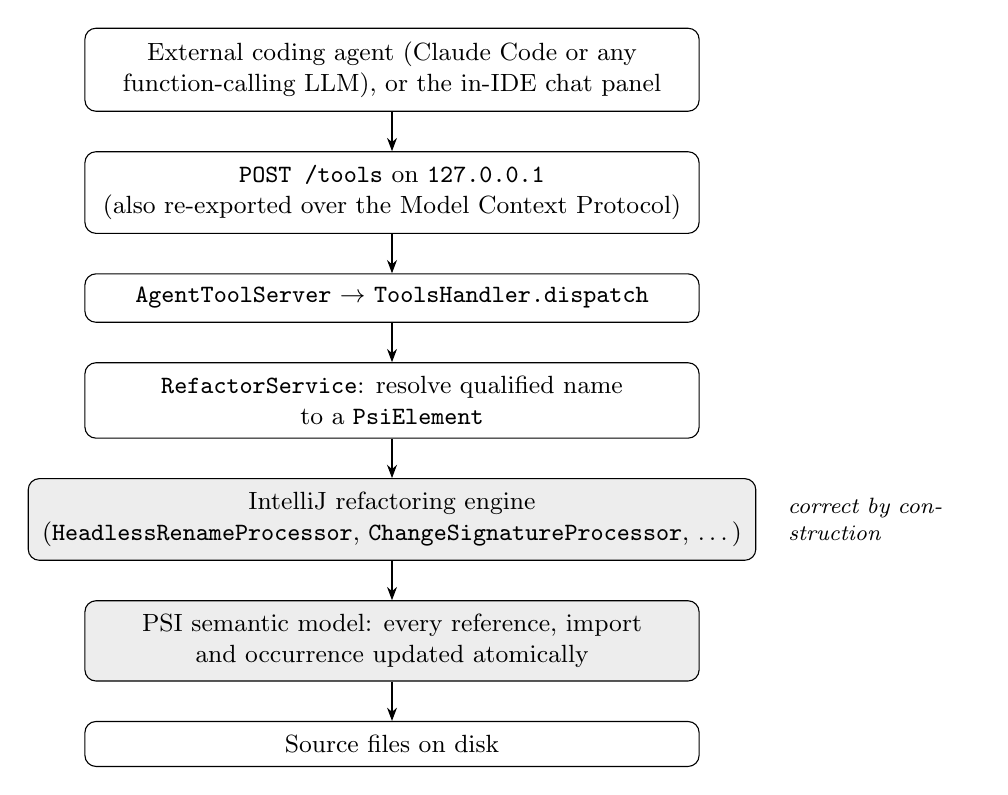
\begin{tikzpicture}[
  font=\small,
  box/.style={draw, rounded corners, align=center, inner sep=5pt, minimum width=78mm},
  eng/.style={box, fill=black!7},
  >={Stealth[]},
  node distance=5mm,
]
  \node[box] (agent) {External coding agent (Claude Code or any\\ function-calling LLM), or the in-IDE chat panel};
  \node[box, below=of agent] (http) {\texttt{POST /tools} on \texttt{127.0.0.1}\\ (also re-exported over the Model Context Protocol)};
  \node[box, below=of http] (server) {\texttt{AgentToolServer} $\rightarrow$ \texttt{ToolsHandler.dispatch}};
  \node[box, below=of server] (svc) {\texttt{RefactorService}: resolve qualified name\\ to a \texttt{PsiElement}};
  \node[eng, below=of svc] (proc) {IntelliJ refactoring engine\\ (\texttt{HeadlessRenameProcessor}, \texttt{ChangeSignatureProcessor}, \ldots)};
  \node[eng, below=of proc] (psi) {PSI semantic model: every reference, import\\ and occurrence updated atomically};
  \node[box, below=of psi] (files) {Source files on disk};
  \foreach \a/\b in {agent/http,http/server,server/svc,svc/proc,proc/psi,psi/files}
    \draw[->] (\a) -- (\b);
  \node[right=3mm of proc, font=\footnotesize\itshape, text width=23mm, align=left] {correct by construction};
\end{tikzpicture}
\caption{Request path from an agent's tool call to a correct-by-construction edit.}
\label{fig:arch}
\end{figure}

As a concrete trace, a rename begins as a call naming the target by qualified name
and a new identifier; the service resolves the name to a \texttt{PsiElement},
hands it to \texttt{RenameProcessor}, and the processor updates the declaration
and every resolved reference across the project as a single atomic refactoring.
In code, the request lands in \texttt{ToolsHandler.handle}, which parses the JSON body
and routes it through \texttt{dispatch} to the project-scoped \texttt{RefactorService}
(resolved via \texttt{project.service<RefactorService>()}). For the rename above,
\texttt{RefactorService.renameByQualifiedName} resolves the name to a
\texttt{PsiElement} and runs a \texttt{HeadlessRenameProcessor} --- a
\texttt{RenameProcessor} subclass that suppresses the otherwise-blocking preview and
conflict dialogs (\Cref{ch:impl}) --- whose \texttt{run()} performs the project-wide
update inside a single write action before the change is flushed to disk. The hosting
\texttt{AgentToolServer} registers \texttt{ToolsHandler} at \texttt{/tools} alongside
\texttt{SchemaHandler} (\texttt{/tools/schema}) and \texttt{StatusHandler}
(\texttt{/status}), all bound to \texttt{127.0.0.1}.

\section{The Tool API Surface}
\label{sec:design-tools}

The API exposes twenty-four operations, grouped by role
(Table~\ref{tab:tools}). All are published as a single JSON schema at
\texttt{GET /tools/schema}, which the agent loads to discover what it can do.

\begin{table}[h]
\centering
\caption{The tool surface, grouped by role.}
\label{tab:tools}
\begin{tabular}{@{}lll@{}}
\toprule
Group & Tools & Correctness basis \\
\midrule
Lookup     & find-symbol-by-name, list-symbols, find-symbol & PSI symbol resolution \\
Refactor   & rename, safe-delete, move-class, change-signature & IntelliJ processors \\
Hierarchy / Inline & pull-up-member, push-down-member, make-static, & IntelliJ processors \\
           & migrate-type, inline-field, inline-method & \\
Create (Java)   & add-field, add-method, add-inner-class, create-file & \texttt{PsiElementFactory} \\
Create (Kotlin) & add-property, add-function, create-file & \texttt{KtPsiFactory} \\
Extract    & extract-method, extract-variable & headless \texttt{MethodExtractor} \\
Inspect    & read-file, find-usages & PSI reference index \\
\bottomrule
\end{tabular}
\end{table}

The Hierarchy/Inline group (pull-up and push-down member, make-method-static,
type-migration, and field/method inlining) is implemented and exposed through the same
schema but is not exercised by the benchmark suites of \Cref{ch:eval}, which concentrate
on the rename, move, change-signature, safe-delete, and usage-discovery core; benchmarking
these higher-level operations is noted as future work (\Cref{sec:concl-future}).

The granularity is chosen to match the unit at which IntelliJ actually guarantees
correctness: one tool per \emph{refactoring operation}. A single coarse
\texttt{refactor} tool would push the hard part --- deciding \emph{which} semantic
operation a request implies --- back onto the model, reintroducing the ambiguity the
design exists to remove. A surface of dozens of fine-grained, PSI-node-level edits
would, in the limit, recreate text editing one node at a time and forfeit the
by-construction guarantee, since correctness in IntelliJ is a property of whole
operations (\texttt{RenameProcessor}, \texttt{MoveClassesOrPackagesProcessor},
\texttt{ChangeSignatureProcessor}), not of individual node mutations. The
operation-level surface also matches what the benchmark tasks actually demand: each
task corresponds to one or two named operations, so the agent completes it by issuing
those operations directly rather than by planning a sequence of low-level edits.

\section{Symbol Resolution by Qualified Name}
\label{sec:design-symbols}

Prior agents address code by file position or byte offset, which forces the model
to guess locations and re-guess after each edit. This design instead addresses
symbols by \emph{qualified name} --- for example \texttt{com.example.Foo\#bar} ---
so the agent operates in the semantic domain of names rather than positions.
Overloaded methods are disambiguated by typed signature: a call naming
\texttt{Owner\#getPet(String,boolean)} resolves to exactly one of three
\texttt{getPet} overloads, and the rename touches only that one and its callers.
This is precisely what the \texttt{pc-rename-method-002} task isolates
(\Cref{sec:eval-rootcause}): renaming only the two-argument
\texttt{Owner\#getPet(String,boolean)} overload while the other two \texttt{getPet}
overloads must survive. The three overloads are lexically identical, so a tool that
matches on the \emph{name} alone cannot tell them apart --- the scripted baseline
renames all three and is caught by the surviving-symbol check. Resolving the target by
typed signature instead lets the engine select exactly the intended overload and
rename it together with precisely its callers, by construction; a text-level approach
can reach the same outcome only by reconstructing, from the surrounding code, the
type information that the signature already carries.

\section{Model-Agnostic Access via MCP}
\label{sec:design-mcp}

To make the model-agnostic claim concrete, a bridge re-exports the HTTP tool API
as a Model Context Protocol server over stdio. It fetches \texttt{/tools/schema}
live, so any tool added to the plugin appears automatically to connected clients,
and any MCP-capable agent (for example Claude Desktop or the Gemini CLI) can drive
the same structured backend with no change to the plugin. This realises the core
architectural separation of the project: the language model is a replaceable
planning layer, and the IntelliJ PSI engine is the execution layer.

\section{Design Alternatives}
\label{sec:design-alternatives}
The design followed fairly directly from the gap analysis of
Chapter~\ref{ch:background} rather than from a wide search over competing
architectures. Several alternative designs nonetheless exist at the key decision
points, and it is worth stating why the chosen approach is preferable to each.

\paragraph{Generate a text patch, then validate it.} A natural alternative keeps the
model generating modified source text and adds a compiler or linter pass afterwards to
reject bad patches. This still places unsafe text generation on the write path: a
compile check catches edits that fail to build, but not edits that compile yet are
semantically wrong --- the over-eager overload rename of \Cref{sec:eval-rootcause}
compiles and would pass such a gate. It also presupposes a build-feedback loop, which
the structured engine does not need, since its edits are correct by construction.

\paragraph{Keep the model inside the IDE, with no external interface.} EM-Assist and
similar tools embed the model in the IDE and expose no callable API. That forecloses
the central contribution --- a model-agnostic surface that \emph{any} external
function-calling agent (Claude Code, the Gemini CLI, or a benchmark harness) can drive
--- and ties the system to a single in-IDE assistant. Exposing the engine over HTTP and
MCP is what makes the execution layer reusable and independently testable.

\paragraph{Address code by position rather than by name.} Prior agents locate targets
by file offset, which the model must guess and then re-guess after each edit shifts the
offsets, and which cannot distinguish overloaded methods. Addressing symbols by
qualified, signature-typed name (\Cref{sec:design-symbols}) keeps the agent in a stable
semantic namespace and lets the engine resolve exactly one overload --- the property
the \texttt{pc-rename-method-002} task exercises (\Cref{sec:eval-rootcause}).

% =============================================================================
%  CHAPTER 4 — IMPLEMENTATION
%  RUBRIC: Execution & Technical Quality (50%). BUDGET: ~8-12 pages.
%  DETAILED OUTLINE (facts from your README / PROJECT_CONTEXT.md / EVALUATION.md).
%  Expand into prose IN YOUR OWN WORDS. Go DEEP on the hard parts (the two
%  engineering challenges) — depth over breadth is what reaches the 70-84 band.
%  Include short, well-explained code listings (lstlisting), not whole files.
% =============================================================================
\chapter{Implementation}
\label{ch:impl}

\section{Plugin Structure and the Tool Server}
\label{sec:impl-server}
% OUTLINE:
%   - AgentToolServer.kt: starts an HTTP server on 127.0.0.1:6473 when a project opens.
%   - Endpoints: POST /tools (ToolsHandler dispatch), GET /tools/schema (SchemaHandler,
%     Claude-compatible tool defs), GET /status (StatusHandler).
%   - Dispatch: ToolsHandler maps {tool, params} -> a project service method.
%   - Threading: PSI mutations must run on the EDT inside a write action; describe
%     the runProcessorOnEdt dispatcher used by the refactoring processors.
%   - Key source files (one line each): RefactorService.kt, PsiCreationService.kt,
%     KotlinCreationService.kt, ProjectContextProvider.kt, ApiKeyService.kt.
\texttt{AgentToolServer} starts a \texttt{com.sun.net.httpserver.HttpServer} bound to
\texttt{127.0.0.1:6473} when a project opens (via a \texttt{StartupActivity}) and
registers three contexts: \texttt{POST /tools} (\texttt{ToolsHandler}),
\texttt{GET /tools/schema} (\texttt{SchemaHandler}, which serves the function-calling
tool definitions), and \texttt{GET /status} (\texttt{StatusHandler}). A request carries
a JSON body \texttt{\{tool, params\}}; \texttt{ToolsHandler.dispatch} maps the tool name
to a method on a project-scoped service --- \texttt{RefactorService},
\texttt{PsiCreationService}, or \texttt{KotlinCreationService}.

The one threading subtlety is that IntelliJ PSI mutations must run on the
event-dispatch thread (EDT) inside a write action, whereas the HTTP request arrives on
a server thread. Each mutating call is therefore marshalled through a small dispatcher,
\texttt{runProcessorOnEdt}, which first waits for indexing to finish
(\texttt{DumbService.waitForSmartMode}), then \texttt{invokeAndWait}s on the EDT,
committing open documents before running the operation and committing and saving all
documents afterwards so the change is flushed to disk before the HTTP response returns.
Simpler, non-processor writes use a sibling dispatcher that wraps the body in a
\texttt{WriteCommandAction}. This is what lets a stateless HTTP call drive a stateful,
thread-confined IDE engine safely.

\section{Refactoring Operations via IntelliJ PSI}
\label{sec:impl-refactor}
% OUTLINE:
%   - Each operation delegates to an IntelliJ processor:
%       rename        -> RenameProcessor
%       move class    -> MoveClassesOrPackagesProcessor
%       change sig    -> ChangeSignatureProcessor
%       safe delete   -> SafeDeleteProcessor
%       inline        -> InlineMethodProcessor
%   - WORKED EXAMPLE (pick rename): trace renameByQualifiedName from the HTTP
%     request, through resolveQualifiedName -> PsiElement, to RenameProcessor.run(),
%     to the updated files. Show the ~5-line core as a listing.
Every refactoring operation is a thin delegation to the corresponding IntelliJ
processor: rename to \texttt{RenameProcessor}, move to
\texttt{MoveClassesOrPackagesProcessor}, change-signature to
\texttt{ChangeSignatureProcessor}, safe-delete to \texttt{SafeDeleteProcessor}, and
inline to \texttt{InlineMethodProcessor}. The service contributes symbol resolution and
headless execution; the processor contributes the correctness guarantee.

A rename is representative. The HTTP layer calls
\texttt{RefactorService.renameByQualifiedName}, whose core is short:
\begin{lstlisting}[basicstyle=\ttfamily\footnotesize]
fun renameByQualifiedName(qualifiedName: String, newName: String, ...): Result {
    refreshProjectFromDisk()                  // reconcile VFS with on-disk state
    val element = ReadAction.compute {
        resolveQualifiedName(qualifiedName) as? PsiNamedElement
    } ?: return Result.Err("could not resolve \"$qualifiedName\"")
    return rename(element, newName, ...)      // runs the processor on the EDT
}
\end{lstlisting}
The qualified name is resolved to a \texttt{PsiNamedElement} inside a read action;
\texttt{rename} then constructs a \texttt{HeadlessRenameProcessor} --- a
\texttt{RenameProcessor} subclass that runs without the interactive preview and
conflict dialogs that would otherwise block an unattended IDE --- and calls
\texttt{run()} inside \texttt{runProcessorOnEdt}. The processor rewrites the declaration
and every resolved reference across the project as a single atomic refactoring before
the files are saved.

\section{Headless Extract-Method}
\label{sec:impl-extract}
% OUTLINE:
%   - Prior extract-method tools (e.g. EM-Assist) are editor-bound: they need an
%     open editor with a caret selection.
%   - This uses IntelliJ's newImpl MethodExtractor.extractMethod(ExtractOptions),
%     driven from a PsiFile + text range with no UI.
%   - Note why this is non-trivial (building ExtractOptions without an editor).
Extract-method is the one operation with no clean headless entry point. The
user-facing refactoring is editor-bound --- tools such as EM-Assist require an open
editor with a caret selection --- because the public API threads an \texttt{Editor}
through option-gathering and the confirmation UI. This plugin instead drives IntelliJ's
\texttt{newImpl} extraction pipeline directly from a file and a text range, with no
editor: \texttt{ExtractSelector().suggestElementsToExtract(psiFile, range)} identifies
the PSI elements covered by the selection, \texttt{ExtractMethodPipeline.findAllOptionsToExtract}
computes the candidate \texttt{ExtractOptions}, and the first option --- with its
\texttt{methodName} replaced by the requested name --- is handed to
\texttt{MethodExtractor().extractMethod(options)} on the EDT. The non-trivial part is
assembling a valid \texttt{ExtractOptions} (the extracted parameters, return type, and
target) without the editor that normally supplies that information; the \texttt{newImpl}
structures expose exactly the entry points needed to do so, where the legacy
extract-method handler does not.

\section{Symbol Creation (Java and Kotlin)}
\label{sec:impl-create}
% OUTLINE:
%   - Java creation via PsiElementFactory (+ auto-format): add_field/method/inner_class/file.
%   - Kotlin creation via KtPsiFactory: add_kt_property/function, create_kotlin_file.
%   - One schema, two languages, no duplication in the HTTP surface; Kotlin tools
%     load only when the Kotlin plugin is present.
Creation tools add new code rather than transform existing code, and are built on the
PSI element factories. The Java tools (\texttt{add\_field}, \texttt{add\_method},
\texttt{add\_inner\_class}, \texttt{create\_java\_file}) build elements with
\texttt{PsiElementFactory} and reformat them into the target class or file; the Kotlin
tools (\texttt{add\_kt\_property}, \texttt{add\_kt\_function},
\texttt{create\_kotlin\_file}) do the same through \texttt{KtPsiFactory}. Both languages
are exposed through one JSON tool schema, so an agent works against a single uniform
surface regardless of language. The Kotlin tools are resolved lazily and advertised only
when the Kotlin plugin is present, so the system degrades gracefully to a Java-only
surface when it is not, rather than failing.

\section{Project Context Injection}
\label{sec:impl-context}
% OUTLINE:
%   - ProjectContextProvider builds a system prompt each chat turn containing:
%     project name + source roots, open file(s) with full symbol listings
%     (names, kinds, signatures, offsets), tool-usage + qualified-name guidance.
%   - Effect: the agent is productive on a project it has never seen, with no
%     manual paste of file paths or offsets.
For an agent to act on a project it has never seen, it must discover what is there
without the user pasting file paths or offsets. \texttt{ProjectContextProvider} assembles
this automatically: on each turn it builds a context block containing the project name
and source roots, a symbol listing for the relevant file(s) --- names, kinds,
signatures, and offsets --- and short guidance on the tool surface and on addressing
symbols by qualified name. Because the agent receives the resolved symbol inventory up
front, it can issue a correct \texttt{rename\_symbol} or \texttt{find\_usages} call by
name on its first turn instead of spending turns reading files to locate a target,
which is what makes it productive on an unfamiliar codebase out of the box.

\section{Engineering Challenges}
\label{sec:impl-challenges}
% These two subsections are your strongest depth signal — write them fully.

\subsection{VFS Staleness After External File Changes}
\label{sec:impl-vfs}
% OUTLINE (from EVALUATION.md "Plugin robustness fix"):
%   - Symptom: initial structured runs scored 6/8 due to cross-task contamination.
%   - Root cause: git resets between tasks updated the DISK, but IntelliJ's
%     in-memory Documents retained the previous task's state; saveAllDocuments()
%     then silently failed (IntelliJ detected an external-change conflict and
%     refused to overwrite).
%   - Fix: every mutating entry point (renameByQualifiedName, safeDeleteByQualifiedName,
%     moveClass, changeSignature, inlineMethod, extractMethod, extractVariable) and
%     every PSI-creation entry point (addField, addMethod, addInnerClass) now calls a
%     synchronous refresh(false, true) on the source roots before reading PSI.
%   - Why it matters: robustness to external changes (git, external editors, CI) is a
%     property a production plugin needs anyway.
% --- AI FIRST DRAFT from your EVALUATION.md notes. Edit freely; then I polish. ---
The benchmark harness exposed a subtle but consequential interaction between
IntelliJ's in-memory model of a file and that file's state on disk. To keep each
benchmark task independent, the runner commits the project's baseline state
before a task and performs a \texttt{git reset} back to that commit afterwards,
so the next task begins from an identical starting point. Early structured runs
nevertheless scored only 6 of 8 tasks, and the failures were not reproducible in
isolation: a task that failed inside a full run passed when executed on its own.

The cause was a divergence between two representations of the same file. A
\texttt{git reset} rewrites the file on disk, but IntelliJ continues to hold an
in-memory \texttt{Document} reflecting the \emph{previous} task's edits. When the
plugin then applied a refactoring and called \texttt{saveAllDocuments()},
IntelliJ detected that the on-disk file had changed beneath its stale
\texttt{Document}, treated this as an external-modification conflict, and
silently declined to overwrite the file. The refactoring had executed correctly
against the PSI, but its result was never persisted --- so the validation step,
which compiles the project from disk, saw stale contents and reported a failure.

The fix makes every entry point defensive against external changes. Each mutating
operation (\texttt{renameByQualifiedName}, \texttt{safeDeleteByQualifiedName},
\texttt{moveClass}, \texttt{changeSignature}, \texttt{inlineMethod},
\texttt{extractMethod}, \texttt{extractVariable}) and each creation operation
(\texttt{addField}, \texttt{addMethod}, \texttt{addInnerClass}) now performs a
synchronous \texttt{refresh(false, true)} of the project's source roots before it
reads the PSI, forcing IntelliJ's virtual file system to reconcile with disk so
that all subsequent work proceeds from the current contents. With this change the
cross-task contamination disappeared and the suite scored 8 of 8.

Although the bug surfaced through the benchmark's reset-between-tasks pattern, the
underlying requirement is general: a plugin that exposes refactoring operations to
an external agent must tolerate the file system changing beneath it --- through
Git operations, an external editor, or a CI step --- rather than assuming it is
the sole writer. Refreshing before each operation is therefore not a
benchmark-specific workaround but a correctness property a production plugin needs
regardless.

\subsection{Class Rename Must Trigger File Rename}
\label{sec:impl-filerename}
% OUTLINE (from EVALUATION.md "Class rename now guarantees file rename"):
%   - Symptom: renaming a public class updated references in memory but did NOT
%     rename Foo.java -> Bar.java.
%   - Root cause: the initial implementation used manual PSI text replacement
%     (handleElementRename + setName), which skips IntelliJ's file-rename side effect.
%   - Fix: route through RenameProcessor(project, element, newName,
%     searchInComments, searchTextOccurrences).run() (the same runProcessorOnEdt
%     dispatcher used by the other processors), making the file rename part of the
%     same atomic refactoring.
%   - Tie to benchmark task pc-rename-002 (CrashController -> PanicController),
%     validated by compile_and_file_exists (PanicController.java exists).
% --- AI FIRST DRAFT from your EVALUATION.md notes. Edit freely; then I polish. ---
A second defect concerned the gap between renaming a \emph{symbol} and renaming
the \emph{file} that declares it. The initial implementation of class rename
manipulated the PSI directly, calling \texttt{handleElementRename}/\texttt{setName}
to change the class identifier and update its references in memory. For most
symbols this is sufficient; but a public Java class must reside in a file of the
same name, so renaming the class must also rename \texttt{Foo.java} to
\texttt{Bar.java}. The manual PSI path updated the declaration and its usages but
silently skipped this file-rename side effect, leaving a \texttt{PanicController}
class inside a file still called \texttt{CrashController.java} --- which does not
compile.

The fix routes class rename through IntelliJ's \texttt{RenameProcessor}
(\texttt{RenameProcessor(project, element, newName, searchInComments,
searchTextOccurrences).run()}), invoked through the same
\texttt{runProcessorOnEdt} dispatcher already used for moves and signature
changes. Because \texttt{RenameProcessor} models the rename at the level the IDE
itself uses, the file rename happens as part of the same atomic refactoring
rather than as a separate step the plugin must remember to perform.

This case is captured directly by benchmark task \texttt{pc-rename-002} (renaming
\texttt{CrashController} to \texttt{PanicController}), whose validation was
deliberately changed from a RefactoringMiner check to
\texttt{compile\_and\_file\_exists}: it asserts that \texttt{PanicController.java}
exists at the expected path after the operation, a direct and observable signal
that the file rename actually occurred. It also illustrates the project's central
thesis in miniature: delegating to the IDE's own refactoring engine yields a
correct, whole-operation result --- declaration, references, and file together
--- whereas the manual approach reproduced exactly the kind of partial,
inconsistent edit that a text-level tool would produce.

% =============================================================================
%  CHAPTER 5 — EVALUATION
%  SOURCE:   docs/EVALUATION.md + docs/CROSS_AGENT_EVALUATION.md + results/*.json
%  RUBRIC:   Evaluation & Reflection (20%) + heavy Execution (50%) overlap
%  BUDGET:   ~10-14 pages — this chapter earns the most marks per page.
%  TOP BAND: fair baselines, measured (not predicted) numbers, explicit threats
%            to validity, and self-critical interpretation.
%
%  >>> THE #1 RISK (see memory project-evaluation-gap):
%      - Do NOT present the 4 petclinic "PASS (expected)" rows as results.
%      - Do NOT headline scripted-regex baseline vs predicted-structured as the
%        main correctness claim — it is not apples-to-apples.
%      - RUN the structured Claude agent AND the LLM text-edit agent on the
%        9-task petclinic suite, then report THOSE numbers.
%
%  >>> WHAT IS DRAFTED HERE (AI first draft, grounded in your docs — verify every
%      number against results/*.json, then edit into your own voice):
%        - Research Questions, Experimental Setup, Validation Methodology
%        - Sample-project results table (MEASURED: results/structured-4.json vs
%          results/text-edit-1.json)
%        - spring-petclinic scripted baseline (MEASURED 6/9) + root-cause analysis
%        - Threats to Validity (descriptive)
%      WHAT IS YOURS TO WRITE (marked \writeme — the judgement/interpretation):
%        - the Discussion's interpretive claims
%        - the LLM-vs-LLM petclinic numbers slot (run finishing in background)
% =============================================================================
\chapter{Evaluation}
\label{ch:eval}

% --- AI FIRST DRAFT from docs/EVALUATION.md. Edit into your own voice. ---
This chapter evaluates the central claim of the project: that performing
refactorings through the IDE's structured engine, rather than by generating
modified source text, yields transformations that are correct with respect to
the program's semantic model, and does so more efficiently than a text-editing
agent. \Cref{sec:eval-rqs} restates the research questions and maps each to an
experiment. \Cref{sec:eval-setup,sec:eval-validation} describe the benchmark
projects, agents, and the multi-layer validation pipeline that produces the
objective correctness signal. \Cref{sec:eval-sample,sec:eval-petclinic} report
measured results on a small purpose-built project and on the real-world
\texttt{spring-petclinic} application respectively, and \Cref{sec:eval-rootcause}
analyses \emph{why} the text-editing baseline fails the cases it fails.
\Cref{sec:eval-threats} states the threats to validity, and \Cref{sec:eval-discussion}
interprets what the results do and do not establish.

\section{Research Questions}
\label{sec:eval-rqs}
% --- AI FIRST DRAFT. These mirror the RQs you frame in the Introduction; keep
%     the wording consistent with sec:intro-rqs once you write that section. ---
The evaluation is organised around three research questions; a fourth,
concerning developer-perceived effort, is a controlled human study deferred to
future work (\Cref{ch:conclusion}).

\begin{description}
  \item[RQ1 (Correctness).] Does refactoring through the structured IDE engine
    produce semantically correct, compile-safe transformations, and where does a
    text-substitution agent operating on the same tasks fail? \emph{Answered by
    the compile-and-content validation across both benchmark projects
    (\Cref{sec:eval-sample,sec:eval-petclinic}) and the root-cause analysis
    (\Cref{sec:eval-rootcause}).}
  \item[RQ2 (Autonomy).] Can a function-calling LLM, given only the tool API and
    injected project context, complete multi-step refactoring tasks on an
    unfamiliar codebase without manual intervention? \emph{Answered by the
    end-to-end agent runs in which the model is told only the task description and
    must locate symbols and select operations itself.}
  \item[RQ3 (Efficiency).] At equal correctness, does the structured action space
    reduce the interaction cost --- API round-trips and tool invocations --- of
    completing a task relative to raw file editing? \emph{Answered by the turn and
    tool-call measurements in \Cref{sec:eval-sample}.}
\end{description}

\section{Experimental Setup}
\label{sec:eval-setup}
% --- AI FIRST DRAFT from docs/EVALUATION.md §2-5 + CROSS_AGENT_EVALUATION.md. ---

\subsection{Benchmark Projects}
Three Java projects are used. The first, \emph{sample-java-project}, is a Maven
project of ten classes (Java~17) that was constructed specifically to exercise
cross-file refactoring: several tasks rename or move a symbol that is referenced
from other files, so that a tool which updates only the declaration --- and not
its remote references --- produces code that no longer compiles. Because the
project is hand-crafted to expose the structural advantages of AST-aware
refactoring, it functions as a controlled instrument rather than a representative
sample; this is revisited in \Cref{sec:eval-threats}.

The second, \texttt{spring-petclinic}, is the canonical Spring Boot sample
application (cloned at tag \texttt{3.3.0}), comprising roughly thirty classes
organised into the layered packages typical of a real Spring project. It is used
to test whether the agent can navigate an unfamiliar, idiomatic codebase it was
not designed around, and to surface structural hazards --- name collisions across
classes, implicit same-package references, and method overloading --- that a
small artificial project does not naturally contain.

The third, \texttt{commons-lang} (Apache Commons Lang, cloned at tag
\texttt{rel/commons-lang-3.14.0}), is a widely-used utility library of 246
source files --- roughly an order of magnitude larger than the others and from a
different domain. It is included specifically to test whether the structural
findings hold \emph{at scale} on an independent, real-world codebase, addressing
the external-validity concern that the other two projects raise
(\Cref{sec:eval-threats}).

\subsection{Task Suites}
Each project has a corresponding task suite. \texttt{tasks.json} defines eight
tasks on the sample project spanning seven operation types (field and method
rename, move class, safe-delete, inline method, class creation, add method, and
change signature); five of the eight involve at least one cross-file reference.
\texttt{tasks\_petclinic.json} defines nine tasks on \texttt{spring-petclinic}
across the same operation families, including three tasks
(\Cref{sec:eval-rootcause}) specifically chosen to require type- and
reference-level information that text matching cannot recover. Every task carries
a machine-checkable success specification (\Cref{sec:eval-validation}).

\paragraph{Operation coverage and representativeness.} The benchmarked operations
deliberately span both ends of what coding agents do in practice. The large-scale
empirical study of \citet{agenticrefactoring2025} finds that agent refactorings are
dominated by localized renames and type changes (rename-parameter 10.4\%,
rename-variable 8.5\%, change-variable-type 11.8\%), so the rename-heavy core of the
suite mirrors the most common agent behaviour. Conversely, the structural operations
the suite also includes --- move class, change signature, and
overload-disambiguated rename --- are precisely those the same study reports agents
\emph{avoid} relative to human developers, i.e.\ the higher-level changes where
free-text editing is riskiest. The suite therefore exercises an agent both where it
is already active and where a structurally-safe execution layer could expand what it
can attempt without risking incorrect edits.

\subsection{Agents and Modes}
\label{sec:eval-modes}
The primary comparison is between two \emph{edit primitives} --- the structured
IDE engine versus raw text editing --- not between two language models. To
separate the contribution of the edit primitive from that of the driving model's
capability, the primitives are exercised in a controlled $2\times2$ design
(\Cref{tab:modes}): each is driven by (i)~\emph{no LLM} (a scripted ``direct''
runner), (ii)~a \emph{weak, freely-available} model, and (iii)~a \emph{capable
commercial} agent. Holding the model fixed and varying only the primitive
isolates the action space; holding the primitive fixed and varying the model
isolates capability.

\begin{table}[t]
  \centering
  \caption{Evaluation arms. The \emph{direct} modes isolate the edit primitive
  with no LLM; the \emph{agent} modes add an LLM that receives only the task
  description and must locate symbols and choose operations itself. The capable
  agent is the system's intended deployment (a commercial Claude Code agent
  driving the tools); the weak models establish how each action space behaves
  under limited tool-use capability.}
  \label{tab:modes}
  \begin{tabular}{@{}lll@{}}
    \toprule
    Arm & Edit primitive & Driver (model) \\
    \midrule
    Structured direct          & IntelliJ PSI engine  & none (scripted) \\
    Scripted text-edit         & regex/string rewrite & none (scripted) \\
    Structured agent (capable) & IntelliJ PSI engine  & Claude Opus~4.8 \\
    Structured agent (weak)    & IntelliJ PSI engine  & qwen2.5:7b (local) \\
    Text-edit agent (capable)  & raw file I/O         & Claude Opus~4.8 \\
    Text-edit agent (weak)     & raw file I/O         & llama-4-scout (Groq) \\
    \bottomrule
  \end{tabular}
\end{table}

The \emph{direct} modes execute the predefined operation for each task with no
model in the loop: the structured-direct runner calls the plugin's tool API, and
the scripted text-edit runner applies a word-boundary regex substitution. They
isolate the edit primitive itself --- a lower bound for the text side and a
ceiling check for the structured side --- independently of any model's planning.
The scripted baseline is deliberately weaker than a modern LLM agent; it is
included as a transparent lower bound that exposes exactly what raw name-matching
can and cannot do, not as the headline comparator.

The \emph{agent} modes wrap each primitive in an LLM tool-use loop. The agent
receives only the natural-language task description and the injected project
context (\Cref{ch:impl}), and must itself find the target symbol and issue the
appropriate calls; it is never told file paths or text offsets. The runners are
model-agnostic --- a \texttt{--provider} switch drives Anthropic,
OpenAI-compatible, Groq, and local Ollama endpoints --- which both supports the
model-agnostic architectural claim (\Cref{sec:design-mcp}) and lets the
evaluation run on freely available models.

\paragraph{Capable agent (intended deployment).} The capable arm is
\textbf{Claude Opus~4.8} (model identifier \texttt{claude-opus-4-8}). Because no
paid API budget was available, it was exercised in the form the system is
designed for: a commercial \emph{Claude Code} agent driving the tools, realised
as fresh, \emph{blind} subagents --- one per task, given only the task text and
the live tool schema (\texttt{GET /tools/schema}), with no expected answers and
no knowledge of the success criteria. The structured arm makes all edits through
the tools; the text-edit arm edits files directly with no structured tool
available. Both may run \texttt{mvn compile} and iterate to self-correct,
mirroring a real developer's Claude Code session. Each task is independently
scored by the same objective oracle (\Cref{sec:eval-validation}) and the project
is reset between tasks. This use of Claude throughout --- both to orchestrate the
runs and as the agent under test --- is disclosed in the GenAI declaration; it
demonstrates the intended deployment and the action-space ceiling, and is not an
independent third-party benchmark.

\paragraph{Weak agents (capability floor).} The weak structured arm is
\textbf{qwen2.5:7b} served locally through Ollama (no rate limit); the weak
text-edit arm is Groq-hosted \texttt{meta-llama/llama-4-scout-17b-16e-instruct}.
Both use a 20-turn per-task budget at temperature~0. They establish how each
action space degrades under limited tool-use capability --- which, as
\Cref{sec:eval-discussion} shows, differs sharply between the two primitives.

\paragraph{Reproducibility.} The environment was IntelliJ IDEA Community~2025.1.4
(platform build~251), plugin~v0.2.0, launched via Gradle~8.14.3
\texttt{runIde}; Apache Maven~3.8.5 with Oracle JDK~24.0.2 served as the
compile/validation oracle; Python~3.10.5; Ollama~0.30.2. The headless flag
\texttt{-Dide.performance.skip.refactoring.dialogs=true} (and
\texttt{-Didea.trust.all.projects=true} for unattended runs) makes the
refactoring engine non-interactive. Exact commands, model identifiers, and the
per-arm harness are recorded in the project repository
(\texttt{docs/EXPERIMENTAL\_SETUP.md}) so every figure can be reproduced.

\section{Validation Methodology}
\label{sec:eval-validation}
% --- AI FIRST DRAFT from docs/EVALUATION.md §4. ---
Correctness is judged not by inspecting the model's output text but by checking
the state of the project after the operation, through a pipeline of up to four
layers. The key methodological commitment is that \textbf{compilation is the
primary objective correctness signal}: a transformation that misses a cross-file
reference, breaks an import, or renames the wrong symbol manifests as a
\texttt{mvn compile} failure, independently of how plausible the edited text
looks.

\begin{enumerate}
  \item \textbf{Tool-call layer.} Every mutating operation returned success and
    all operations the task requires were actually invoked.
  \item \textbf{Compile layer.} \texttt{mvn compile} succeeds on the project after
    the refactoring. This is the primary signal: it is where an agent that fails
    to update remote references is caught.
  \item \textbf{Disk-content layer.} Task-specific checks on the files on disk:
    that an expected file or symbol exists, or --- for renames and moves --- that
    the \emph{old} symbol name is absent from \emph{all} source files. Content
    checks use a word-boundary regex (\texttt{\textbackslash b<symbol>\textbackslash b})
    so that, for example, \texttt{normalize} does not spuriously match
    \texttt{normalizeInput}. A \emph{surviving-symbol} variant additionally asserts
    that names which \emph{should} have been left untouched are still present,
    which is what catches an over-eager rename (\Cref{sec:eval-rootcause}).
  \item \textbf{RefactoringMiner layer (optional).} For tasks where it applies,
    RefactoringMiner~\citep{refactoringminer2025} is run over the before/after
    commits to confirm that the intended refactoring type (e.g.\ ``Rename Method'',
    ``Move Class'') is detected in the diff.
\end{enumerate}

Both runners enforce \textbf{task isolation}: the project's baseline state is
committed before each task and restored by \texttt{git reset} afterwards, so tasks
cannot contaminate one another. This reset pattern interacts subtly with
IntelliJ's in-memory file model and was the source of one of the engineering
challenges discussed in \Cref{sec:impl-vfs}; the structured runner therefore
forces a virtual-file-system refresh and waits briefly after each reset before
the next task begins.

\section{Results: Sample Project (Measured)}
\label{sec:eval-sample}
% --- AI FIRST DRAFT. Numbers MEASURED and verified against:
%       results/structured-4.json   (structured agent, 8 tasks)
%       results/text-edit-1.json    (text-edit agent, 8 tasks)
%     Recompute before submission if you re-run. ---
On the eight-task sample suite, both agents complete all tasks: the project
compiles and every content check passes in both the structured and the text-edit
modes (\Cref{tab:sample-correctness}). \textbf{On a project of this size,
correctness alone does not separate the two approaches.} A capable LLM driving raw
file edits can compensate for the absence of a reference index by reading every
file and enumerating the call sites by hand --- and on ten classes it has the
context budget to do so.

\begin{table}[t]
  \centering
  \caption{Sample project (8 tasks): correctness and efficiency. Correctness is
  identical; the separation is in interaction cost. Source:
  \texttt{results/structured-4.json}, \texttt{results/text-edit-1.json}.}
  \label{tab:sample-correctness}
  \begin{tabular}{@{}lcc@{}}
    \toprule
    Metric & Structured agent & Text-edit agent \\
    \midrule
    Tasks passed (compile + content) & \textbf{8/8} & \textbf{8/8} \\
    Mean turns (API round-trips) per task     & 3.4 & 4.2 \\
    Mean tool calls per task                  & 3.8 & 9.8 \\
    Median tool calls per task                & 3   & 9.5 \\
    \bottomrule
  \end{tabular}
\end{table}

The separation is instead in \emph{efficiency}. The structured agent completes
each task in fewer API round-trips (mean 3.4 vs 4.2) and substantially fewer tool
calls (mean 3.8 vs 9.8). The mean understates the typical gap, because it is
inflated by a single structured outlier: \texttt{inline-001}, which inlines a
method across five call sites, took 13 structured tool calls. Excluding that task,
the structured agent never exceeds three calls; the \emph{median} of three calls
versus 9.5 is the more representative figure. The mechanism is direct: a
structured rename is one call that updates the declaration and every reference
atomically, whereas the text-edit agent must list files, read several of them,
locate each occurrence, and issue a separate edit per site --- roughly a
$2.6\times$ increase in tool invocations for the same outcome.

For RQ3, this is the trade-off in the structured engine's favour: at equal correctness,
performing the change in a single tool call --- rather than listing files, reading
several of them, and issuing one edit per site --- substantially cuts the agent's
interaction cost. Operationally this matters, because frontier models of the kind behind
Claude Code are metered by tokens and round-trip latency, so fewer calls mean lower cost
and faster completion; and because each discrete operation is a chance to emit a
malformed call or miss a site, fewer operations also mean fewer opportunities to err.

\section{Results: spring-petclinic}
\label{sec:eval-petclinic}
% =============================================================================
%  >>> ACTION REQUIRED before this section is final:
%      1. LLM text-edit petclinic run is executing now ->
%         results/text-edit-petclinic-gptoss.json. Fill tab:petclinic with its
%         per-task PASS/FAIL once it lands.
%      2. Structured-LLM (and remaining structured-direct) petclinic tasks need
%         the sandbox IntelliJ. Until run, DO NOT report them as measured —
%         the table below marks them "not yet run".
% =============================================================================
The sample project shows that a small codebase does not discriminate the two
approaches on correctness. The purpose of \texttt{spring-petclinic} is to test
the correctness claim where it should bite: on an unfamiliar, real-world project
containing structural hazards a ten-class project does not.

\subsection{Scripted text-edit lower bound (measured)}
The scripted text-edit runner --- the no-LLM lower bound --- passes
\textbf{6 of 9} tasks (\Cref{tab:petclinic}). The three failures are not random:
each is a task that requires type or reference information that a word-boundary
text substitution does not have. They are analysed in \Cref{sec:eval-rootcause}.
This establishes, concretely and reproducibly, that raw name-matching is
\emph{insufficient} for three common refactorings on a real codebase --- before
any LLM is involved.

\begin{table}[t]
  \centering
  \caption{spring-petclinic (9 tasks), all columns measured. Scripted text-edit is the
  no-LLM lower bound (\texttt{results/text-edit-petclinic-direct-7.json}); LLM text-edit is
  the \texttt{llama-4-scout} agent (\texttt{results/text-edit-petclinic-llama4scout.json});
  structured executes the plugin's IntelliJ PSI refactoring operations directly, with no
  LLM (\texttt{results/structured-petclinic-direct-FINAL.json}). The structured column is
  the tool-layer ceiling; an LLM-driven structured agent is left to future work
  (\Cref{ch:conclusion}).}
  \label{tab:petclinic}
  \begin{tabular}{@{}llccc@{}}
    \toprule
    Task & Operation & Scr.\ text-edit & LLM text-edit & Structured \\
     & & {\footnotesize(no LLM)} & {\footnotesize(LLM planner)} & {\footnotesize(direct, no LLM)} \\
    \midrule
    \texttt{pc-rename-001}        & rename field      & PASS & PASS & PASS \\
    \texttt{pc-add-method-001}    & add method        & PASS & PASS & PASS \\
    \texttt{pc-find-usages-001}   & find usages       & PASS & \textbf{FAIL}$^\dagger$ & PASS \\
    \texttt{pc-read-file-001}     & read file         & PASS & PASS & PASS \\
    \texttt{pc-rename-002}        & rename class+file & PASS & PASS & PASS \\
    \texttt{pc-rename-method-001} & rename method     & \textbf{FAIL} & PASS & PASS \\
    \texttt{pc-move-001}          & move class        & \textbf{FAIL} & \textbf{FAIL} & PASS \\
    \texttt{pc-rename-method-002} & rename overload   & \textbf{FAIL} & \textbf{FAIL} & PASS \\
    \texttt{pc-change-sig-001}    & change sig.       & PASS & PASS & PASS \\
    \midrule
    \multicolumn{2}{@{}l}{\textbf{Total}} & \textbf{6/9} & \textbf{6/9} & \textbf{9/9} \\
    \bottomrule
  \end{tabular}

  \smallskip
  {\footnotesize $^\dagger$\,The text-edit toolset exposes no structural
  find-usages operation, so the agent cannot answer a project-wide reference query
  by construction.}
\end{table}

\subsection{LLM text-edit agent (measured)}
The LLM text-edit agent shown here --- the \emph{weak} free model
\texttt{llama-4-scout}, driven by raw file tools only (the \emph{capable} text-editing
agent is compared separately in \Cref{sec:eval-controlled}) --- also passes
\textbf{6 of 9} tasks (\Cref{tab:petclinic}), but it is instructive
that it fails a \emph{different} set from the scripted baseline. The agent
\emph{succeeds} on \texttt{pc-rename-method-001}, the cross-class \texttt{addVisit}
collision that defeats the scripted substitution: by reading the relevant files it
renames only \texttt{Owner.addVisit} and its caller while leaving
\texttt{Pet.addVisit} untouched, which the surviving-symbol check confirms. A
capable model can therefore reason its way past a name collision that pure string
matching cannot. It likewise renames the class \emph{and} its file correctly in
\texttt{pc-rename-002}.

It nonetheless fails exactly where text editing lacks information the IDE engine
has by construction. On \texttt{pc-move-001} it moves \texttt{PetValidator} to the
new package (the file appears at the new path) but the project no longer compiles,
because it does not synthesise the now-required import for the same-package
reference to \texttt{Pet}. On \texttt{pc-rename-method-002} it renames the target
overload to \texttt{findPet} but again breaks compilation. And it cannot perform
\texttt{pc-find-usages-001} at all: the text-edit toolset exposes no structural
usage query, so a project-wide reference count lies outside its action space.

The decisive observation is the \emph{intersection of failures}. The two tasks
that defeat \emph{both} a na\"ive script \emph{and} a capable LLM editing raw text
--- \texttt{pc-move-001} and \texttt{pc-rename-method-002} --- are precisely those
that require synthesising an implicit import and performing an overload-safe rename
with caller updates. These are not the kind of failure a larger model would
obviously remove; they are failures of the \emph{edit primitive}, which acts on
text rather than on a typed, project-wide reference graph
(\Cref{sec:eval-rootcause}).

\paragraph{A practical constraint worth recording.} Running an LLM text-edit agent
over a real project is token-intensive: each turn resends the growing transcript of
file contents the agent has read. A first attempt using a larger model
(\texttt{gpt-oss-120b}) on a free API tier could not complete the suite at all ---
its per-minute token limit (8{,}000) is exceeded once one or two source files are
in context, so six of nine tasks aborted before any edit was made. The run reported
here used a model whose free-tier per-minute budget (30{,}000 tokens) was large
enough to sustain the loop. The structured agent never reads whole files into the
prompt to act on them (\Cref{sec:eval-sample}), so its per-task token footprint is
far smaller --- an efficiency advantage with a direct cost dimension.

\subsection{Structured operations (measured)}
Executing the same nine tasks through the plugin's IntelliJ refactoring operations
yields \textbf{9 of 9} (\Cref{tab:petclinic}). Decisively, the structured engine
passes every task that defeats one or both text approaches, and the validation
signals confirm \emph{why}:
\begin{itemize}
  \item \texttt{pc-move-001}: \texttt{PetValidator} is moved to the \texttt{system}
    package and the project still \emph{compiles} --- \texttt{MoveClassesOrPackagesProcessor}
    synthesised the import for the same-package reference to \texttt{Pet} that the
    text agents could not (\Cref{sec:eval-rootcause}).
  \item \texttt{pc-rename-method-002}: only the \texttt{(String, boolean)} overload
    becomes \texttt{findPet}; the surviving-symbol check confirms the other
    \texttt{getPet} overloads are untouched --- the type-signature targeting that
    text matching lacks.
  \item \texttt{pc-rename-method-001}: \texttt{Owner.addVisit} becomes
    \texttt{recordVisit} while \texttt{Pet.addVisit} survives, and
    \texttt{pc-rename-002} renames the class \emph{and} its file on disk.
\end{itemize}
Against these baselines the headline is \textbf{structured 9/9 versus 6/9 for both
text approaches}, with the gap concentrated in exactly the three reference-graph /
type-system operations of \Cref{sec:eval-rootcause}. Two qualifications are essential,
and are developed in \Cref{sec:eval-controlled}. First, this column isolates the
\emph{edit primitive}: it executes the operations directly, with no LLM planner, and so
measures whether the structured tools \emph{can} perform each task correctly --- which
they do by construction. That an LLM can itself \emph{select and invoke} these
operations correctly is confirmed by running the structured \emph{agent} (Claude
Opus~4.8) end-to-end: it also scores 9/9 here, and 4/4 and 3/3 on the two larger
projects (\Cref{sec:eval-controlled}) --- so the LLM-driven structured agent is now
\emph{measured}, not deferred. Second, the ``6/9 for text'' figure is for the scripted
baseline and a \emph{weak} free model; a \emph{capable} text-editing agent does
markedly better (7/9), so the durable claim is not raw correctness against any text
editor but the action space's behaviour under limited capability, together with the
structural queries and precision that text editing cannot match.

\paragraph{Engineering the structured runner to be non-interactive (and a threat to
validity).} Driving IntelliJ's refactoring engine unattended is not free: the engine
is built for an interactive user, so multi-file operations raise modal dialogs (a
usage preview, a conflicts dialog, an automatic-rename dialog) that block the UI
thread indefinitely when no one is present to dismiss them. Reaching the 9/9 above
required making the operations genuinely headless --- routing them through the
platform's non-interactive code paths (the \texttt{ide.performance.skip.refactoring.dialogs}
switch and proceeding past recorded conflicts) and ensuring each operation resolves
an in-project element after reconciling the virtual file system with the on-disk
state. This is the same external-change hazard analysed in \Cref{sec:impl-vfs},
encountered again here: the benchmark git-resets the project between tasks, and a
stale virtual file system manifested as refactorings that executed in the PSI but
did not persist, or as ``element is not located inside the project'' precondition
errors. This is on-thesis rather than incidental: the structured numbers were obtained
on a freshly imported, isolated IDE instance, and making the headless path robust ---
suppressing the modal dialogs and reconciling the virtual file system after each
git-reset (\Cref{sec:impl-vfs}) --- was itself an engineering result rather than
something the platform provided for free. It is a fair counter-cost to record against
the approach: the structured engine's correctness guarantee comes with the burden of
driving a UI-oriented IDE unattended.

\subsection{Diff Minimality}
\label{sec:eval-diff}
% --- AI FIRST DRAFT. Numbers measured + instrumented:
%       results/structured-petclinic-direct-DIFF.json  (structured)
%       results/text-edit-scripted-DIFF.json           (scripted text-edit)
%       results/text-edit-petclinic-DIFF.json          (LLM text-edit; only 2 tasks
%         completed before the Groq free-tier daily token cap). ---
Beyond pass/fail, the \emph{size} of the change a refactoring produces matters for
reviewability; small, surgical diffs are easier to audit, and
\citet{agenticrefactoring2025} note that agent refactorings are valued for being
localized. Instrumenting the runners to record the source-line delta of each task
(\Cref{tab:diff}) shows structured execution is consistently the more surgical.
Across the seven mutating petclinic tasks the structured engine changes a median of
8 lines (mean 8.3, 58 in total), against the scripted text-edit baseline's median 12
(mean 21.7, 152 in total --- roughly $2.6\times$ more); the LLM text-edit agent, on
the two tasks it completed before exhausting the free API tier's daily token budget,
likewise rewrote more (17 vs 10 lines for the field rename, 6 vs 3 for add-method).

\begin{table}[t]
  \centering
  \caption{Source-line delta per task (lines changed\,/\,files touched). Structured
  and scripted text-edit are complete; the LLM text-edit agent (\texttt{llama-4-scout})
  completed only two tasks before the free-tier daily token cap (the rest are omitted
  rather than counted as zero). Read-only tasks (find-usages, read-file) change
  nothing and are excluded.}
  \label{tab:diff}
  \begin{tabular}{@{}lccc@{}}
    \toprule
    Task & Structured & Scripted text-edit & LLM text-edit \\
    \midrule
    \texttt{pc-rename-001}        & 10\,/\,1 & 12\,/\,1            & 17\,/\,2 (fail) \\
    \texttt{pc-add-method-001}    & 3\,/\,1  & 1\,/\,1            & 6\,/\,1 \\
    \texttt{pc-rename-002}        & 8\,/\,3  & 37\,/\,1           & --- \\
    \texttt{pc-rename-method-001} & 6\,/\,3  & 10\,/\,3 (fail)    & --- \\
    \texttt{pc-move-001}          & 5\,/\,3  & 64\,/\,1 (fail)    & --- \\
    \texttt{pc-rename-method-002} & 8\,/\,2  & 20\,/\,3 (fail)    & --- \\
    \texttt{pc-change-sig-001}    & 18\,/\,6 & 8\,/\,2           & --- \\
    \midrule
    \textbf{Total} & \textbf{58} & \textbf{152} & --- \\
    \bottomrule
  \end{tabular}
\end{table}

The contrast is sharpest on the structural tasks. On \texttt{pc-move-001} the
scripted approach rewrites 64 lines in a single file and still fails to compile,
whereas the structured move touches 5 lines across 3 files and succeeds; on the
overload rename the structured engine changes 8 lines (correct) against the
baseline's 20 (incorrect). The one task where the structured engine changes
\emph{more} lines is \texttt{pc-change-sig-001} (18 lines across 6 files): correctly
propagating a new parameter to every call site legitimately requires touching every
caller. This is the right reading of minimality --- not the fewest lines in the
absolute, but the minimal \emph{correct} change. Structured edits are confined to a
symbol's declaration and its genuine references; text approaches make incidental,
over-broad substitutions that touch more code and, on the structural tasks, break
it. This also bears on \emph{auditability}: a small, structurally-scoped diff, together
with the explicit tool-call trace the agent produces (\Cref{ch:design}), is far easier
for a developer to review and trust than a large free-text rewrite whose intent must be
reverse-engineered from the changed lines.

\subsection{Root-Cause Analysis of the Text-Edit Failures}
\label{sec:eval-rootcause}
% --- AI FIRST DRAFT from docs/EVALUATION.md §7b. This material is strong and
%     fully grounded in the task definitions; verify file/line references. ---
The three scripted failures share a single underlying cause: text-level editing
lacks the reference graph and the type information needed to act on the right
symbol. Each failure isolates one facet of that deficiency.

\paragraph{Cross-class name collision (\texttt{pc-rename-method-001}).}
The task renames \texttt{Owner.addVisit(Integer, Visit)} to \texttt{recordVisit}.
A different class, \texttt{Pet}, independently declares \texttt{addVisit(Visit)}.
The scripted baseline performs a word-boundary substitution of \texttt{addVisit},
which cannot distinguish the two declarations: it also renames \texttt{Pet.addVisit}
and the \texttt{pet.addVisit(visit)} call in \texttt{VisitController}, violating
the task. IntelliJ's \texttt{RenameProcessor} operates on the specific PSI node
for \texttt{Owner.addVisit}; its reference index knows that
\texttt{pet.addVisit(visit)} resolves to \texttt{Pet.addVisit} and leaves it
untouched. The \emph{surviving-symbol} check detects the difference: after the
structured rename, \texttt{addVisit} still appears as \texttt{Pet}'s declaration
and at its call site, whereas after the text-edit rename it has been erased from
every file.

\paragraph{Implicit same-package dependency (\texttt{pc-move-001}).}
\texttt{PetValidator} and \texttt{Pet} both live in the \texttt{owner} package, so
\texttt{PetValidator} references \texttt{Pet} with no \texttt{import} statement;
likewise \texttt{PetController} uses \texttt{PetValidator} without one. Moving
\texttt{PetValidator} to the \texttt{system} package requires two new imports to be
synthesised. The scripted baseline can only rewrite \emph{explicit}, fully
qualified references, so it leaves both files importless and the project fails to
compile (\texttt{cannot find symbol: class Pet}). IntelliJ's
\texttt{MoveClassesOrPackagesProcessor} resolves references through the PSI graph,
which includes same-package references that have no import line, and inserts the
required imports automatically.

\paragraph{Overload collision (\texttt{pc-rename-method-002}).}
\texttt{Owner} declares three overloads of \texttt{getPet}: \texttt{(String)},
\texttt{(Integer)}, and \texttt{(String, boolean)}. The task renames only the
\texttt{(String, boolean)} overload to \texttt{findPet}. The scripted substitution
matches the name \texttt{getPet} and renames all three; the project still compiles
(the renames are internally consistent), so this failure would be \emph{invisible
to a compile-only check} --- it is caught only by the surviving-symbol assertion
that \texttt{getPet} must still be present. IntelliJ resolves the target by typed
signature (\texttt{Owner\#getPet(String,boolean)}) and renames exactly one
overload. This case is the clearest illustration of why compilation alone is a
necessary but not sufficient correctness signal.

\paragraph{Synthesis.} In each case the structured engine succeeds because it acts
on a typed node in a project-wide reference graph, while the text substitution acts
on a name string. The deficiency is not that the baseline is poorly engineered but
that the information it would need --- which class a call belongs to, which
references resolve without an import, which overload a signature selects --- is
simply not present in the text. This is the core argument of the thesis made
concrete: see \Cref{sec:eval-discussion}.

\section{Results: Apache Commons Lang (Second Real Project)}
\label{sec:eval-commons}
% --- AI FIRST DRAFT. Measured: results/commons-lang-structured-DIFF.json (structured,
%     no-LLM, via the sandbox IDE) vs results/commons-lang-scripted-DIFF.json (scripted
%     text-edit). 4-task suite: benchmarks/tasks_commons_lang.json. ---
To test whether the structural findings generalise beyond \texttt{spring-petclinic},
the comparison was repeated on Apache Commons Lang --- an order of magnitude larger
(246 source files) and from an unrelated domain (a general-purpose utility library).
A focused four-task suite targets the two discriminating operations
(\Cref{tab:commons}): an overload-disambiguated rename (rename only the
three-argument \texttt{StringUtils.replace} overload), a cross-class collision
(rename \texttt{ArrayUtils.contains(int[],int)} while \texttt{StringUtils.contains}
must survive), plus a field rename and a find-usages query as controls.

\begin{table}[t]
  \centering
  \caption{Apache Commons Lang (4 tasks), measured. Structured executes the IntelliJ
  PSI operations; scripted text-edit is the no-LLM regex baseline. ``Lines'' is the
  source-line delta of the change (\Cref{sec:eval-diff}).}
  \label{tab:commons}
  \begin{tabular}{@{}llcc@{}}
    \toprule
    Task & Operation & Structured & Scripted text-edit \\
     & & {\footnotesize(direct, no LLM)} & {\footnotesize(no LLM)} \\
    \midrule
    \texttt{cl-rename-field-001}       & rename field       & PASS (32 lines)  & PASS (480 lines) \\
    \texttt{cl-rename-overload-001}    & overload rename    & PASS (356 lines) & \textbf{FAIL} (compile) \\
    \texttt{cl-rename-cross-class-001} & cross-class rename & PASS (422 lines) & \textbf{FAIL} (compile) \\
    \texttt{cl-find-usages-001}        & find usages        & PASS (213 refs)  & PASS (40 grep hits) \\
    \midrule
    \multicolumn{2}{@{}l}{\textbf{Total}} & \textbf{4/4} & \textbf{2/4} \\
    \bottomrule
  \end{tabular}
\end{table}

The outcome replicates the petclinic finding on a far larger, independent codebase:
the structured engine passes all four tasks, while the scripted text-edit baseline
fails both structural tasks at the compile stage. The mechanism is identical to
\Cref{sec:eval-rootcause} --- a word-level substitution of \texttt{replace} also
rewrites \texttt{java.lang.String\#replace} calls, and \texttt{contains} rewrites JDK
\texttt{List}/\texttt{String} calls, so the project no longer compiles --- but the
scale is greater: \texttt{ArrayUtils.contains(int[],int)} is referenced from 56 files,
each of which the structured rename updates correctly and atomically.

Two observations are specific to scale. First, the find-usages query exposes the gap
between structural and textual reference-finding directly: the structured engine
resolves \textbf{213} genuine references to \texttt{CharRange}, whereas the baseline's
grep returns only 40 textual matches --- the structural index is both more complete
and free of false positives. Second, diff size behaves differently from the small
project. On the field rename the structured edit is surgical (32 lines) while the
regex baseline changes \textbf{480} lines --- it substitutes every lexical occurrence
of \texttt{calendar} across the library and still compiles, a vivid illustration of
how a text approach can pass a naive check while making a sweeping, semantically
unwarranted change. For the ubiquitous \texttt{replace} and \texttt{contains} methods,
by contrast, the structured edit is itself large (356 and 422 lines): correctly
updating every caller of a widely-used method legitimately touches many files. The
robust claim at scale is therefore not ``fewer lines'' but \emph{minimal correct
change} --- the structured engine changes exactly the genuine references and nothing
else, whereas the text approach changes a comparable or larger amount incorrectly.
This second real-world project strengthens external validity: the structural
discriminators that defeat text editing replicate on an independent codebase an order of
magnitude larger, and the controlled comparison (\Cref{sec:eval-controlled}) extends the
evidence to a third, larger project (\texttt{jackson-databind}, 474 files). The central
findings therefore rest on three independent real-world codebases, not one.

\section{Controlled Comparison: Holding the Model Constant}
\label{sec:eval-controlled}
The comparisons above pair the structured engine against a \emph{weaker} text side
--- a no-LLM regex script, or a small free model. That leaves a confound: does the
structured engine win because of the action space, or because the text side had a
weaker planner? The final experiment removes the confound by holding the model
fixed --- the capable agent, Claude Opus~4.8 (\Cref{sec:eval-modes}) --- and varying
only the edit primitive, on both real-world projects.

\begin{table}[t]
  \centering
  \caption{Controlled comparison: the \emph{same} capable agent (Claude Opus~4.8)
  driving each edit primitive, scored by the identical oracle. The last column
  excludes the non-refactoring probes --- a project-wide find-usages query in each
  project, plus one read probe --- that text editing cannot express as a structured
  tool call.}
  \label{tab:controlled}
  \begin{tabular}{@{}lccc@{}}
    \toprule
    Project (tasks) & Structured & Text-edit & Refactoring tasks only \\
    \midrule
    spring-petclinic (9)  & 9/9            & 7/9            & 7/7 vs.\ 7/7 \\
    Commons Lang (4)      & 4/4            & 3/4            & 3/3 vs.\ 3/3 \\
    jackson-databind (3)  & 3/3            & 2/3            & 2/2 vs.\ 2/2 \\
    \midrule
    \textbf{Total}        & \textbf{16/16} & \textbf{12/16} & \textbf{12/12} \\
    \bottomrule
  \end{tabular}
\end{table}

This result is reported in full because it \emph{qualifies the headline}. With a
capable model in the loop, the two action spaces are \textbf{indistinguishable on
behaviour-preserving refactoring correctness}: on every rename, move, and
change-signature task --- including the overload-disambiguated and cross-class
renames that defeat the regex baseline, and at the scale of \texttt{jackson-databind}
(a class referenced from 107 files) --- the agent editing raw text reaches the same
compiling, content-correct result as the agent driving the IDE engine. It does so by
supplying for itself the very capability the structured engine externalises: reading
the affected files, enumerating the call sites, and re-compiling to catch its own
mistakes.

The entire measured gap (16/16 vs.\ 12/16) lies in the tasks where text editing has
\emph{no corresponding primitive}: a project-wide \texttt{find\_usages} query in each
of the three projects --- where the text agent can only grep, returning, on Commons
Lang, 40 lexical hits against the structured index's 213 genuine, type-aware
references --- plus one read probe scored on a specific tool call. \textbf{On the
twelve behaviour-preserving refactoring tasks the two action spaces are tied, 12/12}
--- including \texttt{jackson-databind}'s 551- and 349-reference class renames, which
the text agent completed by hand. Against a capable text editor, then, the structured
engine's advantage on \emph{correctness} narrows to the structural \emph{queries} that
text fundamentally cannot perform.

This sharpens, rather than collapses, the thesis. It locates precisely where the
structured action space earns its value:
\begin{itemize}
  \item \textbf{Driver capability.} The correctness advantage is decisive exactly when
  the driver \emph{cannot} compensate by reading and re-compiling. The no-LLM regex
  baseline fails the structural tasks outright (2/4 on Commons Lang,
  \Cref{tab:commons}); it is the capable model's iterative self-correction --- not the
  text primitive itself --- that closes the gap.
  \item \textbf{Correct by construction vs.\ contingently correct.} The structured
  engine is correct in a single pass (it scored 7/9 here even \emph{without} a feedback
  loop). The text agent's parity was obtained \emph{with} a compile-and-fix loop;
  where no build feedback is available, that contingency is what fails.
  \item \textbf{Structural queries.} Exhaustive, type-aware reference finding has no
  text-level equivalent, and is a primitive real refactoring workflows depend on.
  \item \textbf{Operation count and precision.} The structured agent completes each
  refactoring in a single mutating call that touches only the typed references. A
  capable text agent is, perhaps surprisingly, comparably economical in raw
  \emph{operations} --- it renamed the 551-reference \texttt{ClassUtil} across 107
  files with two bulk substitutions and two compile checks. But a bulk substitution
  matches by \emph{name}: it can also rewrite comments, strings, and unrelated
  identifiers that share the name, and ``it compiled'' does not establish that it did
  not (cf.\ the regex baseline's 480-line over-broad rename, \Cref{tab:commons}). The
  structured edit is precise by construction; the text edit is a heuristic that
  happened to be correct here.
\end{itemize}

\section{Threats to Validity}
\label{sec:eval-threats}
% --- AI FIRST DRAFT. Required for the top band; verify each claim holds for your
%     final runs and add/remove threats honestly. ---
\paragraph{Construct validity.} The sample project was \emph{deliberately designed}
to expose cross-file weaknesses of text editing; it is an instrument for isolating
the phenomenon, not a representative codebase, and its results should be read as
such. The \texttt{spring-petclinic} suite mitigates this by using an external,
real-world project the author did not write, but the nine tasks were still chosen
by the author and are not a random sample of maintenance work.

\paragraph{Internal validity.} The scripted text-edit baseline is an intentional
lower bound and does not, on its own, support a claim about LLM agents; the LLM
text-edit agent (\Cref{sec:eval-petclinic}) is the fair comparator and the basis
for any claim about agents. Correctness is measured by compilation plus content
checks rather than by behavioural (test-suite) equivalence, so a change that
compiles and passes the content checks but alters runtime behaviour would not be
caught; the operations evaluated are, however, all behaviour-preserving by
construction in the structured engine.

\paragraph{External validity.} Four projects and one language (Java; Kotlin
symbol-creation is implemented but not benchmarked) are evaluated, over a bounded set
of operation types. Three are real-world codebases the author did not write
(\texttt{spring-petclinic}; Apache Commons Lang at 246 source files; and
\texttt{jackson-databind} at 474), and the controlled capable-agent comparison
(\Cref{sec:eval-controlled}) was run on all three --- so the central findings are
\emph{measured} on independent projects at scale, including class renames touching
107 files, not merely hypothesised. Two caveats remain. The tasks were chosen by the
author rather than sampled randomly from real maintenance history. And correctness is
judged by compilation plus content checks, not behavioural equivalence; in particular,
a capable text agent's bulk substitution can be \emph{over-broad} (rewriting comments
or strings) yet still compile, so the structured engine's precision advantage
(\Cref{sec:eval-controlled}) is only partly captured by a pass/fail compile oracle and
is evidenced separately by diff size (\Cref{sec:eval-diff}).

\paragraph{Model validity.} Agent results may be specific to the models used. The
capable agent is Claude Opus~4.8; the weak arms are qwen2.5:7b (structured) and
\texttt{llama-4-scout} (text-edit). The qualitative pattern was consistent across the
three projects --- the capable agent reaches parity on refactorings via either
primitive, while the action space is decisive for the weak/scripted drivers --- but it
rests on a single capable model.
That said, the architectural claim does not depend on Claude specifically: the tool API
is model-agnostic (\Cref{sec:design-mcp}), so any function-calling model can drive it,
and re-running the capable arm on a second frontier model (for example a GPT-class model
through the OpenAI-compatible provider) is the natural way to confirm the observed
pattern is not specific to one model (\Cref{ch:conclusion}).

\section{Discussion}
\label{sec:eval-discussion}
% --- This section is YOUR interpretation. A scaffold of the factual frame is
%     drafted; the claims and their hedging are yours to own. ---
The measured results support a \emph{refined} version of the original thesis, and
it is worth stating precisely what they do and do not show.

Against the baselines an automated system would otherwise fall back on --- a scripted
text editor, or a small free model --- the structured engine wins clearly on
correctness: 9 of 9 versus 6 of 9 on spring-petclinic, and the same pattern on Apache
Commons Lang (4/4 versus 2/4), with the gap sitting exactly on the reference-graph and
type-dependent tasks. For drivers of that kind --- which is the regime of cheap, local,
or rate-limited automation --- the action space is decisive.

The controlled comparison then adds the honest qualifier. Given a \emph{capable} agent
--- Claude Opus~4.8, with a compile-and-fix loop --- raw text editing reaches the same
compiling, content-correct result on every behaviour-preserving refactoring, tied 12 of
12 across the three projects, even at the scale of jackson-databind, where it renamed a
551-reference class by hand. I therefore do not claim raw-correctness superiority for
the structured engine over a frontier model: the data does not support it, and stating
so plainly is part of the contribution.

What the data \emph{does} support is narrower but solid. First, a project-wide,
type-aware structural query such as exhaustive \texttt{find\_usages} has no text-level
equivalent --- it is the one task the text agent fails in every project, including the
capable run at scale (2 of 3 on jackson-databind, the single miss being precisely that
query). Second, the structured edit is correct \emph{by construction}: it touches only
typed references, never comments or strings, and needs no build-feedback loop, whereas
the capable text agent's parity was \emph{contingent} on having one. Third, it reaches
the result in far fewer, semantically-scoped operations. Crucially, these advantages are
largest exactly where the driving agent is weakest --- scripted, small, or unverified
--- so the value of the structured action space rises as the driver's capability, or its
access to feedback, falls.

One dimension this evaluation leaves open is cost. The efficiency advantage is argued
here from operation counts and token footprint rather than measured directly; a natural
next step is to quantify the tokens consumed and the wall-clock cost of each approach
across several models, which would establish how large the structured engine's cost
advantage actually is and whether it persists as models improve.

% =============================================================================
%  CHAPTER 6 — CONCLUSION, REFLECTION & FUTURE WORK
%  SOURCE:   docs/EVALUATION.md §9 (refined hypothesis), §10 (developer study)
%  RUBRIC:   Evaluation & Reflection (20%)
%  BUDGET:   ~4-6 pages
%  TOP BAND: mature self-critical judgement + broader impact analysed with depth.
%
%  >>> DRAFTED HERE (AI first draft, grounded in your docs — verify, then edit):
%        - Summary of Contributions (calibrated to MEASURED results)
%        - Limitations, Future Work (incl. the RQ4 study design from §10)
%  >>> YOURS TO WRITE (\writeme — these are judgement parts, per your working
%      agreement): Reflection, Broader Impact. Scaffolds are provided to react to.
% =============================================================================
\chapter{Conclusion and Reflection}
\label{ch:conclusion}

% --- AI FIRST DRAFT. Edit into your own voice; verify every claim is MEASURED. ---
This project set out to test a single architectural proposition: that an LLM
agent performing refactoring should be \emph{decoupled} from the act of writing
code --- deciding \emph{what} to change while delegating \emph{how} to the IDE's
structured refactoring engine. \Cref{ch:design,ch:impl} realised this as an
IntelliJ plugin that exposes rename, move, change-signature, safe-delete, inline,
extract, and symbol-creation operations through a localhost tool API that any
function-calling model can drive, and \Cref{ch:eval} evaluated it against a
text-editing baseline.

\section{Summary of Contributions}
\label{sec:concl-contributions}
% --- AI FIRST DRAFT. Calibrate each bullet to what you actually MEASURED. ---
The work makes the following contributions, each substantiated earlier in the
report:
\begin{itemize}
  \item \textbf{A structured-refactoring tool API for LLM agents.} An IntelliJ plugin
    (\Cref{ch:design}--\ref{ch:impl}) that exposes IntelliJ's PSI refactoring processors
    through a model-agnostic, function-calling interface (HTTP and MCP), letting an
    external agent \emph{execute} project-wide refactorings that are correct by
    construction rather than emit text. To the best of our knowledge this is the first
    general-purpose interface of its kind, contemporaneous with the JetBrains MCP server.
  \item \textbf{A headless-execution technique for IDE refactorings.} A method for
    driving \texttt{BaseRefactoringProcessor}-based operations --- and editor-bound ones
    such as extract-method --- fully non-interactively (\Cref{ch:impl}), suppressing the
    dialogs and editor dependencies that otherwise make them uncallable by an unattended
    agent.
  \item \textbf{A reproducible benchmark and a controlled comparison.} A compile-anchored
    validation harness (\Cref{sec:eval-validation}) and task suites over three real-world
    Java projects (\Cref{ch:eval}), including a model-held-constant comparison that
    isolates the edit primitive from the driving model's capability.
  \item \textbf{An empirical characterisation of where the action space matters.}
    Evidence (\Cref{sec:eval-rootcause,sec:eval-controlled}) that text-level editing
    fails on reference-graph- and type-dependent refactorings for scripted and
    weaker-model drivers, that a capable agent reaches parity on those refactorings, and
    that the structured engine's durable advantages are its structural queries,
    correctness by construction, and robustness to the driver's capability.
\end{itemize}

\section{Reflection}
\label{sec:concl-reflection}
% --- YOUR SECTION (judgement). The refined hypothesis in EVALUATION.md §9 is
%     genuinely self-critical — that honesty is what earns marks here. ---
The most valuable part of this project, in retrospect, was being proven partly wrong. I
set out expecting the structured engine to be straightforwardly \emph{more correct} than
text editing, and against the scripted and weak-model baselines it is. But the controlled
comparison refined that into something more honest: a capable model edits text correctly
too, even at scale, when it has a compile-and-fix loop, so the structured engine's
durable advantage is not raw correctness but that it is correct \emph{by construction},
supports queries text cannot express, and needs no such loop. Delegating to IntelliJ's
own processors gave that correctness for free on exactly the cases the baselines failed
--- the part of the design that worked best was the part I wrote least of. Starting
again, I would run the cross-model and behavioural (test-based) validation earlier
rather than leaning on compilation and content checks, since those are the experiments
that would most sharpen the claim.

\section{Broader Impact}
\label{sec:concl-impact}
% --- YOUR SECTION (judgement). Required from the 60% band up. ---
A broader implication of this work is that, as capable agents become commonplace, the
differentiator shifts from the models themselves towards the \emph{infrastructure} they
act through --- the structured, verifiable tool layers that let an agent change the
world reliably rather than by best-effort generation. Framed as a safety property, this
is the value of constraining the action space: a small, typed, correct-by-construction
set of operations is safer than an unconstrained ``edit any text'' action, because whole
classes of silently-wrong change simply cannot be expressed
\citep{demystifying2025, sweagent2024}. The benefit is greatest for \emph{less} capable
models, which cannot reason their way around a missing guarantee --- so this kind of
infrastructure is a route to making cheaper, local, or open models usefully reliable,
not only to making frontier models marginally better. The pattern is not specific to
refactoring: the same argument extends to CAD and engineering tooling, to reliable code
generation, and to the widening range of MCP-exposed tools across domains as different
as travel and design.

This shifts what a developer must verify. When the edit itself is performed by a
semantics-preserving engine, attention moves from ``did the change apply correctly?'' to
``was this the right change to ask for?'' --- a genuine reduction in the surface for
silently-wrong edits to reach a codebase. The same property cuts both ways, however. A
guarantee that the mechanics are correct can encourage \emph{over}-trust, with
developers reviewing agent-applied changes less carefully precisely because they compile
and look safe; and it concentrates influence in whoever builds and controls the tool
layer, since every agent that depends on it inherits its blind spots. Infrastructure
that makes automated change safer also makes large automated change easier --- a
responsibility as much as a capability.

Finally, the efficiency dimension carries a sustainability angle: performing a
refactoring in a single structured operation rather than many file reads and per-site
edits reduces the API round-trips, token cost, and therefore the energy spent per task
--- a small but real consideration as agentic workflows scale up.

\section{Limitations}
\label{sec:concl-limitations}
% --- AI FIRST DRAFT. Keep these honest and aligned with sec:eval-threats. ---
The evaluation has several limitations, stated here so that the contributions are
not overread. The benchmark covers three real-world projects but a single language (Java; Kotlin
symbol-creation is implemented but not benchmarked), and the operation set, while
spanning seven families, is not exhaustive. Correctness is established by compilation
and disk-state checks rather than by behavioural (test-suite) equivalence, so a change
that compiles and passes the content checks but alters runtime behaviour would not be
caught. The original expectation --- that the structured approach's correctness
advantage would \emph{grow} on large codebases, where an LLM can no longer hold every
file in context --- was tested directly (on Apache Commons Lang and jackson-databind, up
to 474 files) and was \emph{not} borne out for a capable agent: such an agent reached
parity even at that scale (\Cref{sec:eval-controlled}), so the structured engine's
advantage lies in structural queries and correctness-by-construction rather than in raw
scale. The agent arms were also driven by a single capable model (Claude Opus~4.8);
confirming that the pattern is not specific to one model is left to future work, as is
the human-factors question.

\section{Future Work}
\label{sec:concl-future}
% --- AI FIRST DRAFT from EVALUATION.md §10. The RQ4 study design is yours; this
%     frames it as planned-not-done. ---
Several directions follow directly from the limitations above.

\paragraph{Controlled developer study (RQ4).} The most direct extension is the
human-factors study the evaluation deferred. The planned design compares three
conditions --- manual IntelliJ refactoring, an in-IDE chat assistant performing
text edits, and the structured-refactoring agent --- on a fixed set of maintenance
tasks performed by 10--15 participants on an unfamiliar Java project, measuring
time to completion, the number of corrective undo actions, and post-task cognitive
load (NASA-TLX), with a short interview probing whether participants trusted each
change without manually verifying it. This would test whether the structural
correctness guarantees translate into measurable gains in developer effort and
trust, which the present, purely technical, evaluation cannot establish.

\paragraph{Cross-model studies.} The scale comparison was carried out as part of this
work --- on Apache Commons Lang and jackson-databind, up to 474 files
(\Cref{sec:eval-controlled}) --- so the open question is no longer scale but
\emph{generality across models}. Re-running the capable-agent arm on other frontier
models (for example a GPT- or Gemini-class model, through the same model-agnostic tool
interface) would establish whether the observed pattern --- parity on refactoring
correctness, with the structured advantage concentrated in structural queries and
by-construction safety --- holds beyond Claude, as the architecture intends.

\paragraph{Broader operation and language coverage.} Several higher-level operations
are implemented but not yet benchmarked (pull-up and push-down member,
make-method-static, type migration); benchmarking these, adding the operations still
missing (e.g.\ extract-interface, encapsulate-field), and exercising the existing Kotlin
support would broaden the claim beyond the rename, move, and change-signature core
evaluated here. \paragraph{IDE-agnostic backend.}
Because the agent interacts only through the tool API, the same interface could in
principle be backed by another language service (e.g.\ an LSP server or a
different IDE), which would generalise the architecture beyond IntelliJ.

\paragraph{Stronger evaluation oracles.} Correctness here is established by
compilation and content checks; two complementary oracles would deepen it. First,
structural-quality analysis with DesigniteJava --- the methodology of
\citet{agenticrefactoring2025} --- would quantify whether structured refactorings
preserve or improve design-smell and complexity metrics, making the results
directly comparable to that study (and testing the expectation that
behaviour-preserving operations introduce no new smells). Second, the
differential-fuzzing approach of \citet{difffuzzing2026} would verify behavioural
equivalence beyond compilation --- a behavioural complement to the structural
guarantees the engine already provides by construction.

My own view is that AI-assisted refactoring should become both more widespread and more
\emph{language-aware}. Most agentic coding today happens at the command line and edits
code as text; the natural next step is to wire these agents, by default, into the
structured engine of whatever language they are working in --- the PSI for Java and
Kotlin, an equivalent service elsewhere --- so that whenever the language is known, edits
flow through its abstract syntax tree rather than through free text. I believe that shift
could meaningfully improve how safely and correctly code is written, precisely as more of
it comes to be written with AI.


% ============================== BIBLIOGRAPHY =================================
\bibliographystyle{plainnat}
\bibliography{references}

% ============================== APPENDICES ===================================
\appendix
\chapter{Tool API Reference}
% Full 24-tool JSON schema, example requests/responses. Good place to move
% detail out of the Implementation chapter to respect the page limit
% (check whether appendices count toward your page limit — see WRITING_GUIDE.md).
The tool surface is published as a single JSON schema served at
\texttt{GET /tools/schema} (the live schema is authoritative; a grouped summary appears
in \Cref{tab:tools}). Each tool is invoked by POSTing a \texttt{\{"tool",\,"params"\}}
body to \texttt{/tools}. Two representative calls follow.

A rename by qualified name:
\begin{lstlisting}[basicstyle=\ttfamily\footnotesize]
POST /tools
{"tool": "rename_symbol",
 "params": {"qualifiedName": "...petclinic.owner.Owner#telephone",
            "newName": "phoneNumber"}}
=> {"ok": true, "message": "renamed telephone to phoneNumber"}
\end{lstlisting}

A project-wide, type-aware usage query (no text-level equivalent):
\begin{lstlisting}[basicstyle=\ttfamily\footnotesize]
POST /tools
{"tool": "find_usages",
 "params": {"qualifiedName": "org.apache.commons.lang3.CharRange"}}
=> {"count": 213, "usages": [{"filePath": "...", "line": 61, "preview": "..."}]}
\end{lstlisting}
The complete operation set, parameters, and return shapes are documented in the live
schema and in the project repository.

\chapter{Benchmark Task Definitions}
Each task in the benchmark suites (\texttt{benchmarks/tasks\_petclinic.json},
\texttt{tasks\_commons\_lang.json}, and \texttt{tasks\_jackson.json}) carries a
natural-language description, the canonical operation(s), and a machine-checkable success
specification. One representative entry --- the overload-safe rename of
\Cref{sec:eval-rootcause} --- is:
\begin{lstlisting}[basicstyle=\ttfamily\footnotesize]
{"id": "pc-rename-method-002",
 "description": "Rename the two-argument overload getPet(String, boolean) in Owner
                 to findPet; do not rename the other getPet overloads.",
 "project": "spring-petclinic",
 "operations": [{"tool": "rename_symbol",
                 "params": {"qualifiedName": "...owner.Owner#getPet(String,boolean)",
                            "newName": "findPet"}}],
 "validation": {"type": "compile_and_symbol_exists",
                "expectedSymbol": "findPet", "crossFileCheck": true}}
\end{lstlisting}
The full suites are available in the project repository.

\end{document}
